% \documentclass[12pt,a4paper]{extbook}
\documentclass[a4paper]{extbook}

\usepackage{scrextend}
\changefontsizes[15pt]{13pt}
% -------- Border Cover
\usepackage {fancybox} % Use this package.
\usepackage{afterpage} % Insert the blank page
\def\blankpage{%
      \clearpage%
      \thispagestyle{empty}%
      \addtocounter{page}{-1}%
      \null%
      \clearpage}
% -------- Header and Footer

% \usepackage{lastpage}
% \usepackage{scrlayer-scrpage}
% \clearscrheadfoot
% \ohead{\headmark}
% \usepackage{calc}
% \cfoot{\thepage / \pageref{LastPage}}


% -------font and Paragraph

\usepackage[utf8]{inputenc}
\usepackage[vietnamese]{babel}
\usepackage{fontspec}
\setmainfont{Times New Roman}
\newfontfamily{\uctimes}{Times New Roman}[
  Mapping=uc-text
]

% -------------- Stype Itemize 
\usepackage{enumitem}
\setlist[itemize]{noitemsep, topsep=0pt}

% \setlist[itemize]{itemsep=10pt, label={--}}
% \setlist[itemize]{itemsep=10pt}
\setlist{  
  listparindent=\parindent,
  parsep=0pt,
  wide=0pt,
}
% ------------ Figure Latex
\usepackage{graphicx,caption,float}
% --------- Chapter style  Font the section and subsection and spacing section

\usepackage{titlesec}
\titleformat{\chapter}[display]
    {\filcenter\normalfont\Large\bfseries}
    % {\MakeUppercase{\chaptertitlename}\ \thechapter}
    % {5pt}
    % {}
    {\MakeUppercase{\chaptertitlename}\ \thechapter}
    {1pt}
    {\MakeUppercase}
    [\vspace{.5ex}\titlerule]

    % ------ 
    \setcounter{secnumdepth}{4}
    
    % ------ 
    \titleformat{\section}
    {\normalfont\fontsize{12}{15}\bfseries}{\thesection}{1em}{}
    \titleformat{\subsection}
    {\normalfont\fontsize{12}{15}\bfseries}{\thesubsection}{1em}{}
    \titleformat{\subsubsection}
    {\normalfont\fontsize{12}{15}\bfseries}{\thesubsubsection}{1em}{}
    \titleformat{\paragraph}
    {\normalfont\normalsize\bfseries}{\theparagraph}{1em}{}
    \titlespacing*{\paragraph}
    {0pt}{3.25ex plus 1ex minus .2ex}{1.5ex plus .2ex}
    
\titlespacing*{\chapter}{0pt}{0pt}{40pt}
\titlespacing*{\section}{0pt}{0pt}{1pt}
\titlespacing*{\subsection}{0pt}{0pt}{1pt}
\titlespacing*{\subsubsection}{0pt}{0pt}{1pt}

% --------- Setting Paragraph
\usepackage{indentfirst}
\renewcommand{\baselinestretch}{1.5}
\setlength{\parskip}{0.3\baselineskip}%set space between paragraphs

% ------------- math 
\usepackage{amsmath,amsfonts,amssymb}
\usepackage[math-style = upright]{unicode-math} %Math equations non italic: https://tex.stackexchange.com/questions/318087/math-equations-non-italic



% --------------- Ki hieu vat li + hoa hoc
\usepackage{physics,mhchem}
\usepackage{siunitx}

% --------------- Bang Table
\usepackage{tabularx,ragged2e,booktabs,multirow,longtable}
\newcolumntype{C}{>{\Centering\arraybackslash}X}
\usepackage[skip=0.333\baselineskip]{caption} % optional


% -------------------------------------------------------
\usepackage[a4paper,left=3.5cm, right=2cm,top=3.5cm,bottom=3cm,asymmetric]{geometry}

% ----------------Table of Contents ToC -------------------------------
\usepackage{tocstyle}
\usetocstyle{standard}


% ----------------Tai lieu tham khao -------------------------------
% --------------- Bookmark, Reference,  Bibligraphy
\usepackage{bookmark,hyperref}
\usepackage[sorting=none]{biblatex}
\addbibresource{Chapter/Reference.bib}
\nocite{*}
% ------------------ TIeu de
\title{Khoá luận 2019}
\author{VU QUANG NGUYEN}

% ---------------------------Start------------------------------------------------------
\begin{document}
% % FIXME: ---------------------------------- Page for Cover

\begin{titlepage}
    \thisfancypage{%
    \setlength{\fboxsep}{10pt}\doublebox}{}
    
    


%% temporary titles
% command to provide stretchy vertical space in proportion
\newcommand\nbvspace[1][3]{\vspace*{\stretch{#1}}}
% allow some slack to avoid under/overfull boxes
\newcommand\nbstretchyspace{\spaceskip0.5em plus 0.25em minus 0.25em}
% To improve spacing on titlepages
\newcommand{\nbtitlestretch}{\spaceskip1cm}
\pagestyle{empty}


\begin{center}
{\nbtitlestretch\normalsize
ĐẠI HỌC QUỐC GIA THÀNH PHỐ HỒ CHÍ MINH\\
TRƯỜNG ĐẠI HỌC KHOA HỌC TỰ NHIÊN\\
KHOA VẬT LÝ – VẬT LÝ KỸ THUẬT\\
NGÀNH KỸ THUẬT HẠT NHÂN}

\nbvspace[1]
------***------\\[1cm]
\bfseries
\normalsize
\nbvspace[1]
\large KHÓA LUẬN TỐT NGHIỆP ĐẠI HỌC\\[4cm]
\normalsize Đề tài:\\
\large QUY TRÌNH XỬ LÝ NHIỄM BẨN PHÓNG XẠ RADIUM TRONG ĐẤT VÀ NƯỚC

\nbvspace[2]


% \includegraphics[width=1.5in]{./graphics/pic37}


\nbvspace[3]
  \bfseries
  \normalsize
\hspace*{5cm}  SVTH: Vũ Quang Nguyên\\
\hspace*{5cm}  CBHD: ThS. Huỳnh Nguyễn Phong Thu\\
\hspace*{5cm}  CBPB : ThS. Huỳnh Nguyễn Phong Thu
\nbvspace[2]



  \bfseries
  \nbvspace[3]
  \nbvspace[2]
  \nbvspace[4]
  \normalsize
  THÀNH PHỐ HỒ CHÍ MINH – 2019
  
\end{center}
\end{titlepage}

% Chen mot trang trong: Da definition  o file header Thesis.tex
\blankpage



% % FIXME: ---------------------------------- Page for Cover


%% temporary titles
% command to provide stretchy vertical space in proportion
\newcommand\nbvspace[1][3]{\vspace*{\stretch{#1}}}
% allow some slack to avoid under/overfull boxes
\newcommand\nbstretchyspace{\spaceskip0.5em plus 0.25em minus 0.25em}
% To improve spacing on titlepages
\newcommand{\nbtitlestretch}{\spaceskip1cm}
\pagestyle{empty}


\begin{center}
{\nbtitlestretch\normalsize
ĐẠI HỌC QUỐC GIA THÀNH PHỐ HỒ CHÍ MINH\\
TRƯỜNG ĐẠI HỌC KHOA HỌC TỰ NHIÊN\\
KHOA VẬT LÝ – VẬT LÝ KỸ THUẬT\\
NGÀNH KỸ THUẬT HẠT NHÂN}

\nbvspace[1]
------***------\\[1cm]
\bfseries
\normalsize
\nbvspace[1]
\large KHÓA LUẬN TỐT NGHIỆP ĐẠI HỌC\\[4cm]
\normalsize Đề tài:\\
\large QUY TRÌNH XỬ LÝ NHIỄM BẨN PHÓNG XẠ RADIUM TRONG ĐẤT VÀ NƯỚC

\nbvspace[2]


% \includegraphics[width=1.5in]{./graphics/pic37}


\nbvspace[3]
  \bfseries
  \normalsize
\hspace*{5cm}  SVTH: Vũ Quang Nguyên\\
\hspace*{5cm}  CBHD: ThS. Huỳnh Nguyễn Phong Thu\\
\hspace*{5cm}  CBPB : ThS. Huỳnh Nguyễn Phong Thu
\nbvspace[2]



  \bfseries
  \nbvspace[3]
  \nbvspace[2]
  \nbvspace[4]
  \normalsize
  THÀNH PHỐ HỒ CHÍ MINH – 2019
  
\end{center}

 
% Chen mot trang trong: Da definition  o file header Thesis.tex
\blankpage
% \clearpage
\tableofcontents
\clearpage

% -------------------Danh so trang La Ma
\pagenumbering{roman}
% -------------------Danh sach bang bieu

\addcontentsline{toc}{chapter}{\listtablename}
\listoftables
\clearpage
% -------------------Danh sach hinh ve

\addcontentsline{toc}{chapter}{\listfigurename}
\listoffigures
\clearpage

% -------------------Danh sach chu viet tat

\addcontentsline{toc}{chapter}{Danh mục các từ viết tắt}
\chapter*{Danh mục các từ viết tắt}


\begin {table}[!htbp]
\begin{center}
    \begin{tabular}{ >{\centering\arraybackslash}m{1.2in}  >{\centering\arraybackslash}m{2.0in} >{\centering\arraybackslash}m{2.5in} }
    \toprule[1.5pt]
    {\bf Từ viết tắt} & {\bf Tiếng Anh} & {\bf Tiếng Việt}\\ 
    \midrule

    RAD7 & Radon Detector-7    &  Đầu dò đo radon-7    \\
    UNSCEAR & United Nations Scientific Committee on the Effects of Atomic Radiation    &  Ủy ban khoa học Liên hợp Quốc về ảnh hưởng bức xạ nguyên tử   \\
   IAEA &  International Atomic Energy  Agency & Cơ quan Năng lượng Nguyên tử Quốc tế\\
   HPGe & High Pure Germanium  & Đầu dò Germani siêu tinh khiết\\
   
    \bottomrule[1.25pt]
    \end {tabular}
\end{center}
\end {table}

\clearpage

% -------------------Loi cam on va mo dau
\addcontentsline{toc}{chapter}{Lời cảm ơn }
\chapter*{Lời cảm ơn}

EM xin gửi lời cảm ơn chân thành này tới các Thầy Cô, đặc biệt là Thầy Cô - Bộ môn Vật lí Hạt nhân và Kĩ thuật Hạt nhân, trường Đại học Khoa học Tự nhiên - ĐHQG TP.HCM, đã tận tình hướng dẫn và giúp đỡ em trong suốt quá trình học tập tại trường.

Em xin chân thành cảm ơn đến Cô Th.S Huỳnh Nguyễn Phong Thu - Phòng thí nghiệm Kĩ thuật hạt nhân đã nhiệt tình và tận tụy, chia sẻ những kiến thức và kinh nghiệm cần thiết trong suốt thời gian thực hiện nghiên cứu đề tài này. Đặc biệt, ngoài trách nhiệm là một cán bộ hướng dẫn đầy trách nhiệm và nhiệt huyết, Cô còn là người thân, luôn quan tâm động viên, chia sẻ những bài học cuộc sống, khuyến khích em vượt qua những khó khăn để hoàn thành tốt khóa luận này. 

Em xin cám Cô PGS. TS. Trương Thị Hồng Loan và Thầy PGS. TS. Lê Công Hảo, đã truyền nhiệt huyến và kinh nghiệm nghiên cứu trong suốt quá trình nghiên cứu khoa học này.

Em xin chân thành cảm ơn tất cả Thầy - Cô  thuộc bộ môn Vật lí Hạt nhân và phòng thí nghiệm Kĩ thuật hạt nhân, đã hướng dẫn tận tình và truyền đạt những kinh nghiệm quý báu, đồng thời hỗ trợ và tạo mọi điều kiện cho em trong suốt quá trình học tập và nghiên cứu. 

Em xin gửi lời cảm ơn sâu sắc đên Thầy Cô trong Hội đồng và giành nhiều thời gian đọc và có những ý kiến đóng góp sâu sắc và thiết thực cho đề tài này được hoàn thiện hơn.

Cuối cùng, em xin gửi lời cám ơn đến gia đình, và bạn bè cùng đồng hành, động viên và khuyến khích em trong quá trình học tập và thực hiện nghiên cứu đề tài này của mình.

Mặc dù, em đã có nhiều cố gắng và nỗ lực cao nhất để hoàn thiện đề tài khóa luận, nhưng không thể tránh khỏi những thiếu sót, rất mong nhận được ý kiến góp ý của Thầy-Cô và các anh chị học viên, em xin chân thành cảm ơn.\\

\hspace*{\fill} TP. Hồ Chí Minh, \today


\addcontentsline{toc}{chapter}{Lời mở đầu }
\chapter*{Lời mở đầu}


Các hoạt động khai thác quặng, dầu và khí tự nhiên, các mạch nước ngầm gây ra phơi nhiễm phóng xạ tự nhiên trong môi trường. Điều này dẫn đến hàm lượng phóng xạ tại các địa điểm diễn ra các hoạt động trên có khả năng vượt ngưỡng an toàn phóng xạ cho phép. Trong số các đồng vị phóng xạ, \ce{^226Ra} được xem là một đồng vị quan trọng do có chu kỳ bán rã dài, khả năng ion hóa cao và có tính chất hóa học tương đồng với nhiều kim loại kiềm thổ khác trong đất. Các đồng vị con cháu của \ce{^226Ra} cũng có có khả năng ion hóa cao, đặc biệt \ce{^226Ra} còn sinh ra 222Rn, một đồng vị phóng xạ dạng khí có khả năng phân tán vào môi trường rất cao ~\cite{IAEANo476:revise}.

Trên thế giới, có nhiều công trình nghiên cứu cho thấy, chất thải tự nhiên do các hoạt động khai thác quặng, dầu khí,...  gây ra có hàm lượng phóng xạ rất cao trong đất, có vùng lên đến 1000 kBq/kg ~\cite{BCR:JamalAlAbdullah}. Do đó, vấn đề đặt ra cho các nhà khoa học là cần xác định mức độ ô nhiễm phóng xạ tại các khu vực này và xây dựng các quy trình chuẩn nhằm giảm thiểu tối đa phơi nhiễm phóng xạ, phục hồi tính trạng môi trường. Nhiều nhà nghiên cứu trên thế giới đã áp dụng phương pháp chiết tách phân đoạn BCR để lọc tách các kim loại nặng trong đất, nổi bật như nghiên cứu của Koguh và cộng sự (1994),  Kozuh  và cộng sự (1996), Mark D. Ho và cộng sự (1997). Phương pháp chủ yếu dựa vào tính chất hóa học, khả năng linh động của các kim loại mà xây dựng quy trình lọc tách phù hợp. Trong khóa luận, chúng tôi áp dụng quy trình chiết tách phân đoạn BCR để chiết tách \ce{^226Ra} từ pha rắn (đất) sang pha lỏng. Đây cũng được xem là một trong những kỹ thuật làm giàu \ce{^226Ra} từ các mẫu có chứa hàm lượng \ce{^226Ra} cao trong môi trường. Trong khóa luận, chúng tôi chưa có mẫu chất thải tự nhiên có hàm lượng \ce{^226Ra} cao. Vì vậy, quy trình lọc tách được áp dụng trên các mẫu đất có hàm lượng \ce{^226Ra} trên mức trung bình thế giới. 

Bên cạnh ô nhiễm phóng xạ \ce{^226Ra} trong đất, các hoạt động khai thác nhiên liệu của con người cũng làm tăng đáng kể nồng độ phóng xạ trong nước ngầm, đặc biệt là \ce{^226Ra}. Tất cả các loại nước sinh hoạt sử dụng hiện nay hầu như đều có nguồn gốc từ nước ngầm. Con người khi tiêu thụ nhiều lượng nước có chứa nồng độ \ce{^226Ra} cao có nguy cơ mắc các bệnh ung thư, đặc biệt là ung thư xương. Vì vậy, việc xử lý nhiễm bẩn phóng xạ trong các nguồn nước ngầm là vấn đề cần thiết trong thực tiễn. Trong khóa luận,  tác giả đã cải tiến phương pháp hấp thụ \ce{^226Ra} bằng sợi tổng hợp polyester tẩm \ce{MnO2} để lọc tách \ce{^226Ra} trong nước giếng dựa trên phương pháp của nhóm Willard S. Moore (1973). Phương pháp cải tiến cho kết quả khả quang: hiệu suất lọc \ce{^226Ra} trong nước từ (80-99\%), và các mẫu  đáp ứng an toàn phóng xạ, liều hiệu dụng về radon và radium đều trong ngưỡng an toàn của UNSCEAR (2000) và USEPA.


Khóa luận được chia thành ba chương:

\textbf{Chương 1}: Trình bày tổng quan về tình hình nghiên cứu trong và ngoài nước liên quan đến mục đích nghiên cứu của khóa luận.Các tính chất vật lí và hóa học của radium, tính linh động, quá trình di chuyển và phân bố của radium trong tự nhiên, ảnh hưởng của radium đến sức khỏe con người cũng như tác động đến môi trường cũng được trình bày trong chương 1.

\textbf{Chương 2}: Trình bày quy trình xác định hàm lượng \ce{^226Ra} trong đất, lọc tách radium trong đất theo quy trình BCR ba bước. Nồng độ radium trong nước được xác định bằng hệ thiết bị RAD7. Quy trình lọc tách \ce{^226Ra} trong nước giếng bằng phương pháp hấp thụ trên MnO2 ⋅ SiO2 được trình bày trong chương này.

\textbf{Chương 3}: Trình bày kết quả lọc tách \ce{^226Ra} trong đất và nước ngầm. Các đánh giá và nhận xét liên quan cũng được trình bày trong chương.


\mainmatter

% -------------------Danh so trang Roman
\pagestyle{plain}
\clearpage
% \chapter{Tổng quan}

\section{Tình hình nghiên cứu về radium trên thế giới}
    \subsection{Các nghiên cứu về radium trong đất và phương pháp chiết tách BCR}

Năm 1997, Mark D. Ho và Greg J. Evans thuộc khoa kĩ thuật hóa học, trường đại học Toroto, Canada đã thực hiện quy trình chiết tách các nguyên tố Cd, Cu, Pb và Zn trong mẫu đất chuẩn NIST bằng quy trình BCR. Hàm lượng các nguyên tố được xác định bằng phương pháp quang phổ hấp thụ khí acetylene. Kết quả cho thấy quy trình chiết tách phân đoạn BCR có khả năng tách được các kim loại nặng Cd, Cu, Pb, và Zn với hiệu suất từ 83 đến 100\% ~\cite{BCR:MarkD.Ho}.

Năm 2000, Nusa Pustisek cùng cộng sự đã áp dụng quy trình chiết tách phân đoạn BCR để tách các nguyên tố Cd, Pb và Zn ra khỏi các mẫu đất thuộc thung lũng Mezica (Slovekia). Đây là khu vực tập trung nhiều nhà máy công nghiệp luyện kim. Hàm lượng của mẫu phân tích trước và sau khi tách chiết được phân tích bằng phương pháp quang phổ nguyên tử hấp thụ. Kết quả phân tích cho thấy, phần trăm chiết tách Cd khá cao khoảng 80\%. Với Pb, hiệu suất đạt khoảng 50\%. Giá trị này đạt 70\% đối với Zn. Hàm lượng của các kim loại nặng trong đất ô nhiễm tại vùng Mezica là rất cao, việc áp dụng quy trình BCR để xử lý nhiễm bẩn kim loại nặng trong đất tại khu vực là vấn đề cấp bách  ~\cite{BCR:OrginNusa}.

Năm 2012, Shigeo Uchida và Keiko Tagami thuộc Viện nghiên cứu quốc gia về phóng xạ Nhật Bản đã đánh giá hoạt độ phóng xạ \ce{^226Ra} trong đất và sự vận chuyển \ce{^226Ra} từ đất vào cây lúa tại 61 điểm ở Nhật Bản. Mẫu đất được nhốt trong 1 tháng để đạt cân bằng phóng xạ \ce{^226Ra} và con cháu và hàm lượng được xác định bằng hệ phổ kế HPGe. Nhóm tác giả đã thực hiện chiết tách \ce{^226Ra} trong gạo bằng phương pháp đồng kết tủa \ce{Ba(Ra)SO4}.  Sau đó, mẫu được nhốt trong 2 tuần và đo bằng đầu dò nhấp nháy lỏng. Kết quả cho thấy: (1) Hoạt độ \ce{^226Ra} trong mẫu đất ở Tây Nam (trung bình 40,4 Bq/kg) cao hơn các mẫu đất tại Đông Bắc (trung bình 27,8 Bq/kg); (2) Hệ số vận chuyển \ce{^226Ra} từ đất vào cây lúa dao động từ 0,07 đến 1,58 ($x10^{-3}$). Hệ số vận chuyển \ce{^226Ra} từ đất vào cây lúa cao hơn so với hệ số vận chuyển từ đất vào rau củ ~\cite{RaSoil:ShigeoUCHIDA}. 

Năm 2013, C. Prieto và cộng sự thuộc trường đại học Salamanca, Tây Ban Nha đã tiến hành nghiên cứu về khả năng rửa giải radium trong đất bằng citrate, EDTA và EDDS. Các mẫu đất được thu thập tại vùng khai thác quặng Los Ratones, Tây Ban Nha. Radium trong các mẫu đất được chiết tách bằng phương pháp đồng kết tủa \ce{Ba(Ra)SO4}, hàm lượng được xác định bằng hệ phổ kế alpha. Hàm lượng \ce{^226Ra} trong đất trung bình đạt 838±108 (Bq/kg). Nhóm tác giả kết luận: (1) Độ rửa giải của radium bằng citrate cao nhất khi nồng độ citrate bằng 50 (mmol/kg). (2) Với EDTA nồng độ 5 (mmol/kg), độ rửa giải radium đạt giá trị cao nhất vào ngày đầu tiên, trong khi đối với citrate, độ rửa giải radium cao nhất vào ngày thứ 4. (3) Với EDDS nồng độ 15 (mmol/kg) tại pH bằng 4, sau 6 ngày, độ rửa giải radium vẫn tiếp tục tăng dần  ~\cite{RaSoil:C.Prieto}.    

Năm 2016, Jamal Al Abdullah cùng cộng sự thuộc Ban an toàn phóng xạ, Ủy ban Năng lượng Nguyên tử Syria đã áp dụng quy trình BCR để chiết tách \ce{^226Ra} ra khỏi đất. Mẫu đất nhiễm phóng xạ \ce{^226Ra} được lấy từ giếng dầu tại Palmya thuộc Syria, hoạt độ phóng xạ \ce{^226Ra} đo được dao động từ $1030 \pm  90$ đến $7780 \pm 530$ (Bq/kg), giá trị trung bình là $2840 \pm 1840$ (Bq/kg). Quy trình chiết tách BCR phù hợp và hiệu quả để chiết tách \ce{^226Ra} trong đất ô nhiễm phóng xạ, giảm nồng độ \ce{^226Ra} trong đất dưới ngưỡng an toàn phóng xạ theo tiêu chuẩn IAEA-2004. Hiệu suất tách chiết \ce{^226Ra} thay đổi đối với các mẫu đất khác nhau, dao động từ 45 đến 99 \% ~\cite{BCR:JamalAlAbdullah}.

Năm 2016, Jamal Al Abdullah cùng cộng sự thuộc Ban an toàn phóng xạ, Ủy ban Năng lượng Nguyên tử Syria đã áp dụng quy trình BCR để lọc tách \ce{^226Ra} ra khỏi đất. Mẫu đất nhiễm phóng xạ \ce{^226Ra} được lấy từ giếng dầu tại Palmya thuộc Syria, hoạt độ phóng xạ \ce{^226Ra} đo được dao động từ $1030 \pm 90$ đến $7780 \pm 530$ (Bq/kg), giá trị trung bình là $2840 \pm 1840$ (Bq/kg). Quy trình chiết tách BCR phù hợp và hiệu quả để chiết tách \ce{^226Ra} trong đất ô nhiễm phóng xạ. Sau khi xử lý, hàm lượng phóng xạ \ce{^226Ra} trong đất giảm dưới ngưỡng an toàn phóng xạ theo tiêu chuẩn IAEA-2004. Hiệu suất lọc tách \ce{^226Ra} thay đổi đối với các mẫu đất khác nhau, dao động từ 45 đến 99 \% ~\cite{BCR:JamalAlAbdullah}.

Quy trình BCR được nhiều nhóm nghiên cứu trên thế giới áp dụng tách chiết các nguyên tố kim loại ra khỏi đất. Một số ít nhóm nghiên cứu đã áp dụng tách chiết phóng xạ. Tuy nhiên, số lượng các nghiên cứu này chưa nhiều, các loại đất ở Việt Nam có thành phần hoàn toàn khác với thành phần đất được khảo sát bởi các nhóm nghiên cứu khác trên thế giới. Vì vậy, vẫn cần có nhiều nghiên cứu liên quan đến hướng nghiên cứu này.



    \subsection{Các nghiên cứu về radium trong nước}

Năm 1975, Moore cùng cộng sự thuộc phòng thí nghiệm phân tích hải dương học Naval, Hoa Kì đã áp dụng phương pháp lọc nước nhiễm phóng xạ \ce{^226Ra} bằng sợi \ce{MnO2}. Các mẫu nước được lấy tại các địa điểm cách vùng Felde (miền nam Texas) từ 300 m – 8 km. Đây là khu vực có nhiều nhà máy tập trung khai thác quặng uranium. Ông đã dùng sợi acrylic tẩm \ce{MnO2} (phần trăm khối lượng của Mn từ 12-15\%) để lọc các mẫu nước thu thập được. Các mẫu nước sau khi lọc đều có lượng \ce{^226Ra} dưới 3 pCi/L, giá trị này nằm trong ngưỡng an toàn theo tiêu chuẩn của Mỹ. Do đó phương pháp lọc radium bằng sợi \ce{MnO2} phù hợp để lọc các nguồn nước mặt, nước ngầm nhiễm phóng xạ radium ~\cite{MnO2:Moore}. 
    
Năm 1979, David F. Reid và cộng sự thuộc bộ môn Hải dương học, trường đại học Texas, Hoa Kì đã tiến hành cải tiến phương pháp hấp thụ radium bằng màng lọc acrylic tẩm \ce{MnO2}. Phương pháp được áp dụng để lọc tách radium, thorium và americium trong nước biển. Kết quả cho thấy màng lọc có hiệu suất tách các đồng vị phóng xạ trong nước biển cao. Đối với radium và actinium, hiệu suất tách bằng màng lọc từ 80-90\% ~\cite{MnO2:DavidFReid}.

Năm 1993, M.T.Crespo và cộng sự cũng áp dụng phương pháp trên để hấp thụ các đồng vị phóng xạ của U, Th, Pu, Am và Ra trong các mẫu nước. Kết quả nghiên cứu cho thấy đối với Ra, hiệu suất hấp thụ đạt từ 87\% đến 97\% trong môi trường trung tính. Trong khi đó, đối với các nguyên tố phóng xạ U, Th, Am và Pu, hiệu suất hấp thụ cao hơn trong môi trường có độ pH thấp ~\cite{MnO2:M.T.Crespo}. 

Năm 1996, Gordana cùng cộng sự thuộc viện nghiên cứu y học và sức khoẻ nghề nghiệp Zegred, Croatia đã tiến hành khảo sát nồng độ \ce{^226Ra} trong nước suối nóng và suối khoáng tại Croatia.  Mẫu nước sau đó được chiết lọc bằng phương pháp đồng kết tủa \ce{BaSO4}.  Nồng độ \ce{^226Ra} trong suối nước khoáng, suối nước nóng và nước giếng dao động từ 0,07 đến 4,40 (Bq/L). Giá trị này vượt quá ngưỡng tiêu chuẩn an toàn của Tổ chức Y tế Thế giới WHO - 2003 là 1 (Bq/L) ~\cite{MnO2:GordanaMarovic}. 

Năm 2003, R.M.R. Almeida cùng cộng sự thuộc khoa Xây dựng, đại học Federal Fluminense, Brazil đã tiến hành khảo sát nồng độ phóng xạ của radium, radon và uranium trong nước ngầm tại Região dos Lagos, Brazil. Các mẫu nước phân tích được lấy tại suối khoáng, nước giếng tại các hộ gia đình. Nhóm nghiên cứu đã áp dụng phương pháp đồng kết tủa radium để xác định nồng độ của \ce{^226Ra} và \ce{^228Ra} trong nước. Nhóm tác giả thực hiện thêm dung dịch \ce{H2SO4} và \ce{BaCl2} vào 1L mẫu nước, để tạo thành phức đồng kết tủa \ce{Ba(Ra)SO4}. Sau đó, tiếp tục hòa tan phức kết tủa trong mẫu bằng cách thêm dung dịch nitrilotriacetic axit (NTA). Cuối cùng, phức đồng kết tủa hòa tan ethylene diamine tetra-acetic acid (EDTA) với pH bằng 10 được dùng để làm sạch. Dung dịch sulphat được kết tủa lại khi thêm axit acetic với pH bằng 4,5 đến 5,0. Radium được tách ra, mẫu được nhốt trong 1 tháng để đạt cân bằng phóng xạ. Nồng độ phóng xạ được đo bằng hệ phổ kế alpha. Nồng độ radium dao động từ dưới 0,01 đến 1,5 (Bq/L), vượt ngưỡng tiêu chuẩn an toàn phóng xạ trong nước sinh hoạt của Brazil (0.1 Bq/L). Suất liều chiếu của người dân sử dụng nguồn nước trong một năm lên tới 0.8 (mSv). Kết quả cho thấy, nồng độ phóng xạ của radium trong nước cao khi pH của dung dịch thấp (dưới 5,5) ~\cite{MnO2:RMRAlmeida}

Năm 2009, Richard N. Peterson cùng cộng sự thuộc bộ môn Hải dương học, trường đại học Florida, Hoa Kì đã tiến hành so sánh các phương pháp xác định nồng độ \ce{^226Ra} trong nước biển. \ce{^226Ra} trong mẫu nước được hấp thụ bằng sợi acrylic tẩm \ce{MnO2}. Các mẫu nước sau đó được xác định hàm lượng \ce{^226Ra} bằng các hệ thiết bị khác nhau, bao gồm RAD7, RaDeCC, hệ đo radon vết và hệ phổ kế gamma HPGe. Kết quả cho thấy sợi \ce{MnO2} hấp thụ cao các đồng vị của radium: \ce{^226Ra}, \ce{^224Ra}, \ce{^223Ra} và \ce{^228Ra}. Tác giả đề nghị tùy theo điều kiện và mục đích nghiên cứu, có thể lựa chọn phương pháp phân tích phù hợp. Hệ đo RAD7 có ưu điểm ghi đo tự động, thời gian nhốt mẫu thấp. Hệ đo radon vết và RaDeCC có hiệu suất ghi cao, thời gian ghi đo và nhốt mẫu thấp phù hợp để ghi đo bức xạ của \ce{^223Ra} và \ce{^224Ra}. Quy trình chuẩn bị mẫu phân tích cho hệ phổ kế gamma khá đơn giản, hệ phổ kế ghi nhận được đồng thời \ce{^226Ra} và \ce{^228Ra} ~\cite{MnO2:RichardNPeterson}.

\section{Các đồng vị của radium trong tự nhiên}

% FIXME: ------------------

Trong tự nhiên, radium chủ yếu có bốn đồng vị chính gồm \ce{^223Ra}, \ce{^226Ra}, \ce{^228Ra} và \ce{^224Ra}, là con cháu của các chuỗi phân rã \ce{^238U}, \ce{^235U} và \ce{^232Th}. Thông tin về các đồng vị của radium được trình bày trong bảng ~\ref{table:RaDecay}. Hình ~\ref{figure:ChainDecay} trình bày sơ đồ phân rã của ba họ phóng xạ tự nhiên. Ba chuỗi phân rã này có một số đặc điểm chung  ~\cite{Thesis:HNPThu}:  

\begin{itemize}
    \item Đồng vị mẹ trong mỗi chuỗi có thời gian bán rã rất dài, gần bằng tuổi Trái đất. Đồng vị \ce{^232Th}, thời gian bán rã dài, $1,4 \times 10^{10}$ năm, hầu như hàm lượng không thay đổi quá nhiều trong thời gian tồn tại của Trái đất. Đồng vị \ce{^238U} có thời gian bán rã $4,9 \times 10^9$ năm, đã bị phân rã một phần, tạo ra nhiều đồng vị con cháu tồn tại trong môi trường.
    \item Mỗi chuỗi phân rã đều có một đồng vị phóng xạ tồn tại dạng khí, là các đồng vị khác nhau của radon. \ce{^222Rn}, \ce{^219Rn} và \ce{^220Rn} lần lượt là các thành viên của chuỗi phân rã \ce{^238U}, \ce{^235U} và \ce{^232Th}. Trong đó, \ce{222Rn} có thời gian bán rã dài nhất, 3,825 ngày, là đồng vị có ý nghĩa nhất trong các nghiên cứu này.  
    \item  Mỗi chuỗi phân rã đều kết thúc bằng các đồng vị bền của chì. Chuỗi \ce{^238U} kết thúc bằng đồng vị \ce{^206Pb}. \ce{^207Pb} và \ce{^208Pb} lần lượt là các đồng vị cuối của các chuỗi phân rã \ce{^235U} và \ce{232Th}.
\end{itemize}


\begin{figure}[htbp]
    \centering 
    \setlength{\fboxsep}{0pt}%
    \setlength{\fboxrule}{0.8pt}%
    \fbox{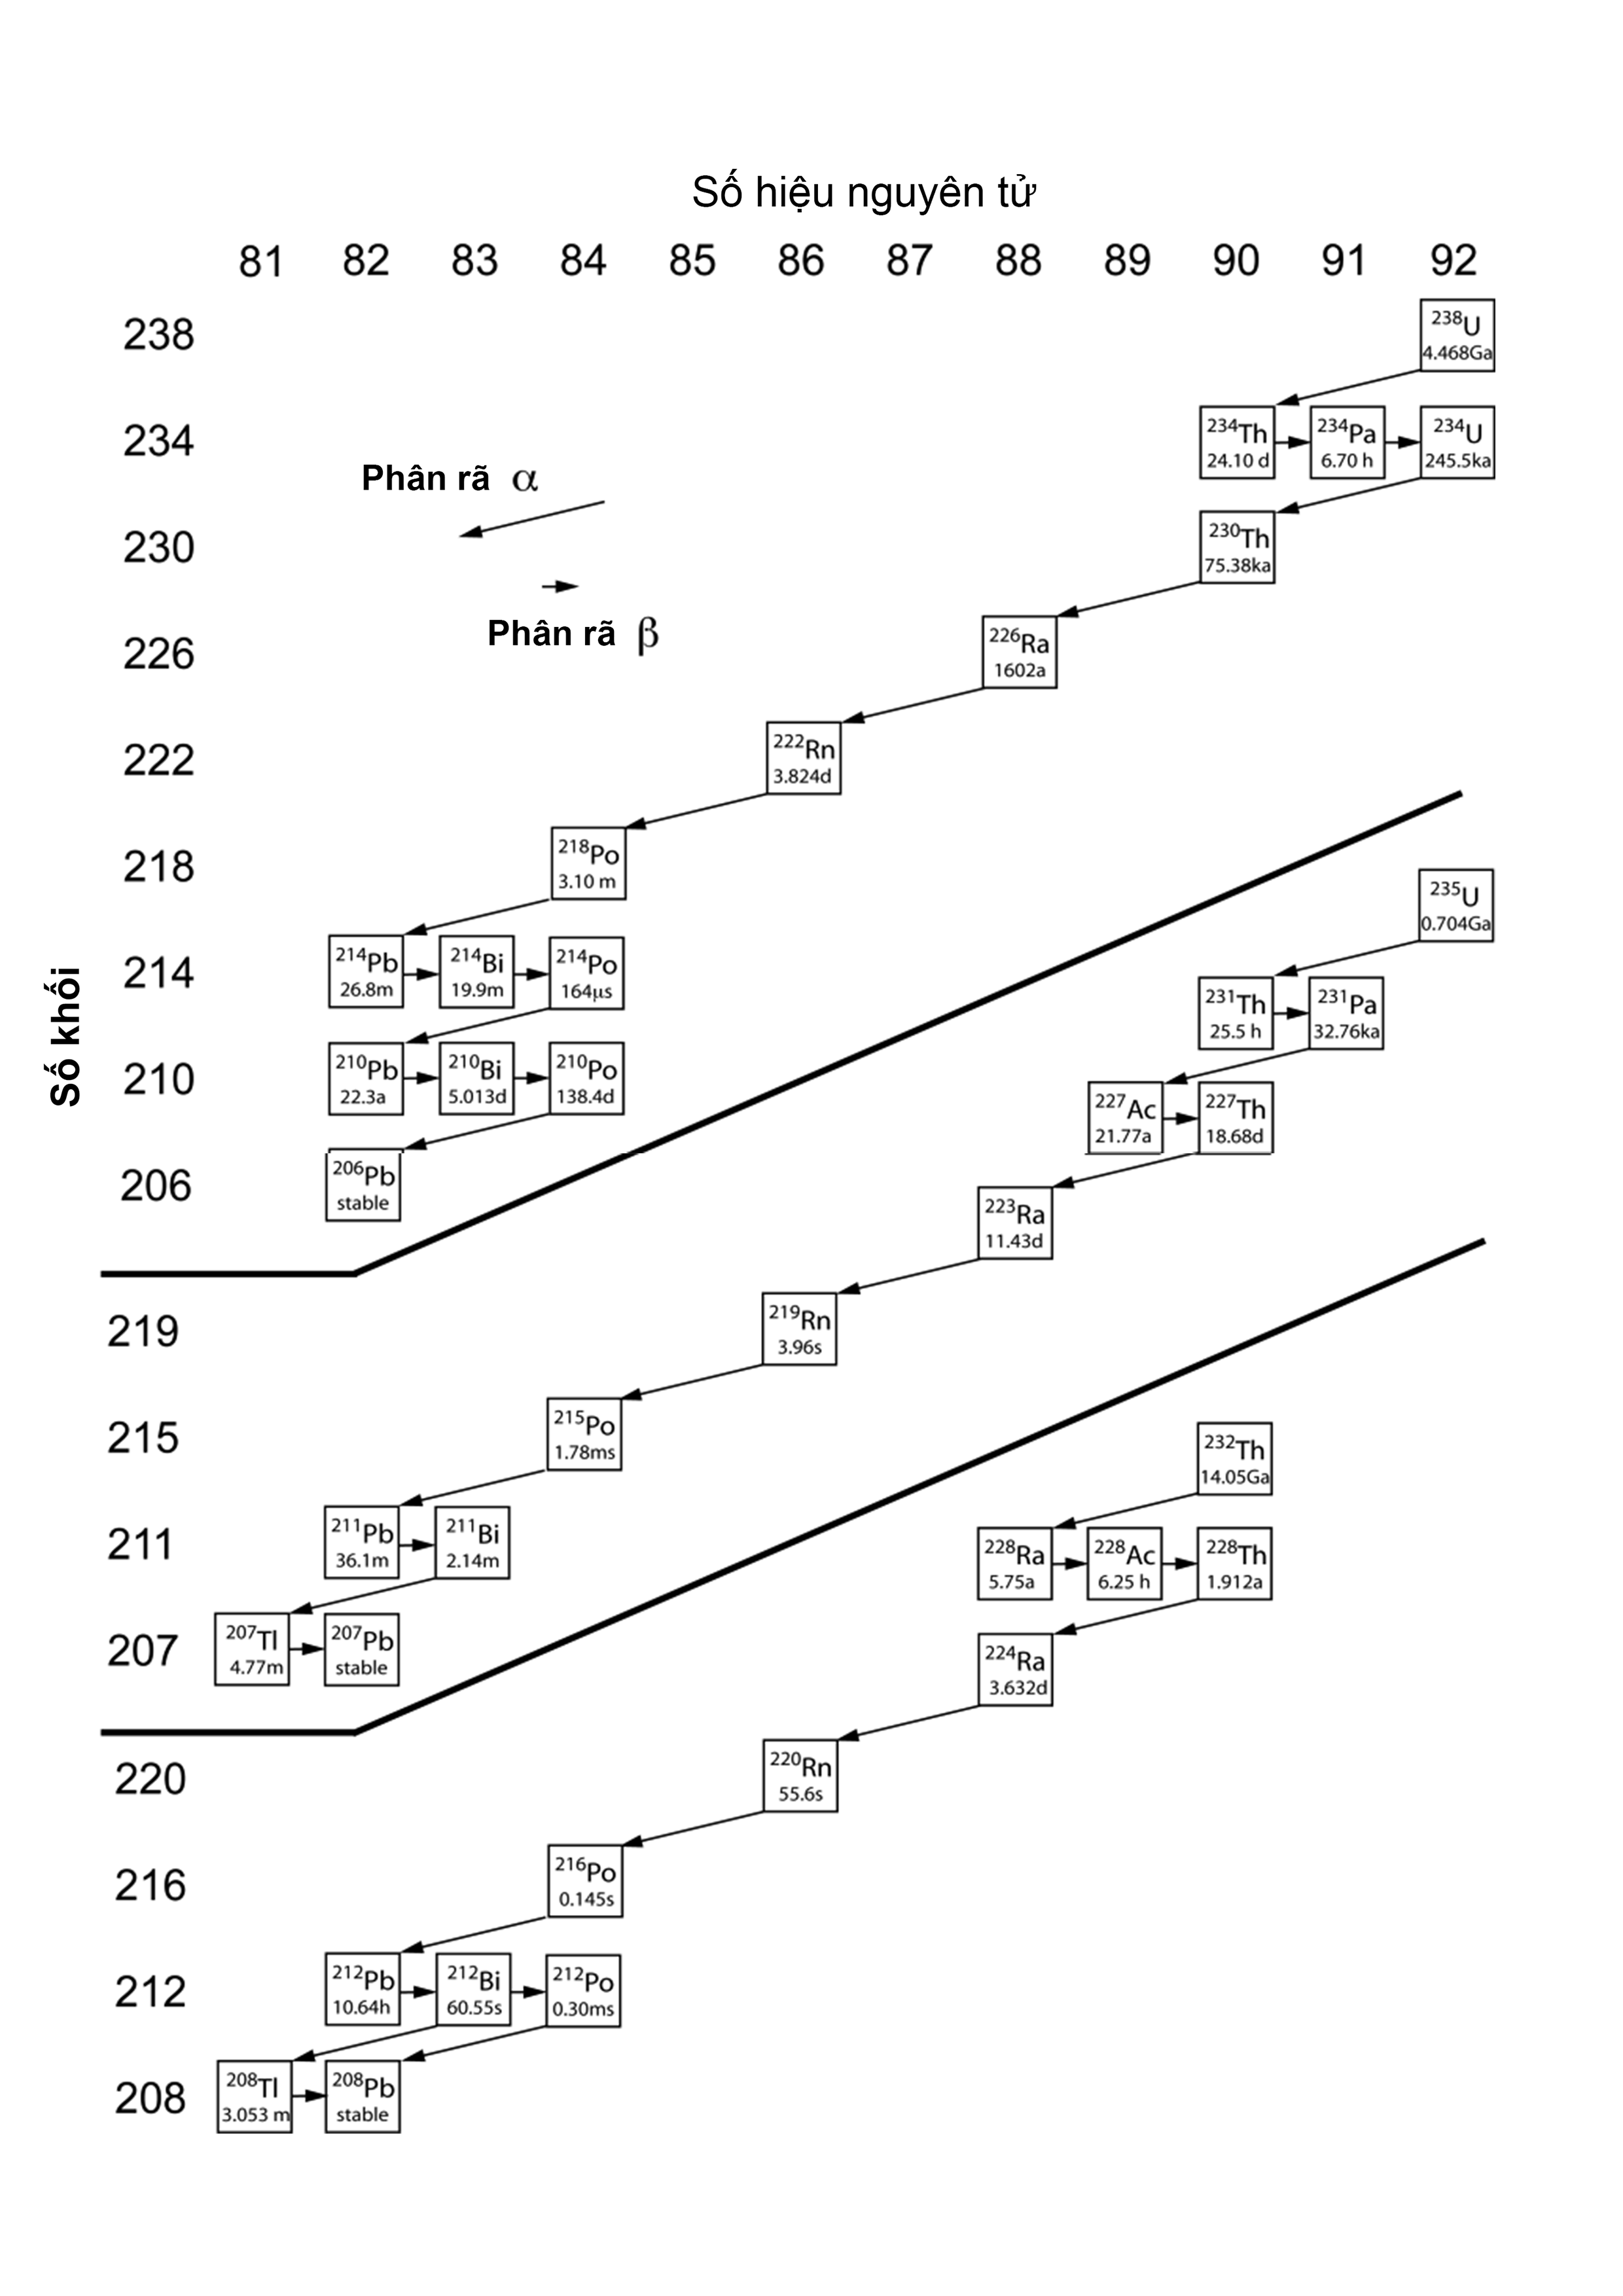
\includegraphics[width=\textwidth]{Image/Chapter1-ChainDacay.png}}
    \caption{Sơ đồ của ba chuỗi phân rã phân rã tự nhiên ~\cite{IAEANo476:revise}}
    \label{figure:ChainDecay}
\end{figure}
 

Các đồng vị của radium thường sử dụng làm chất đánh dấu trong các nghiên cứu liên quan đến địa chất, thủy văn . \ce{^223Ra} có chu kì phân rã dài nhất (1600 năm), độ phộ cập trên 99\%, phát cả bức xạ alpha và gamma trong quá trình phân rã nên được xem là đồng vị phóng xạ tự nhiên nguy hiểm nhất đối với con người và môi trường ~\cite{IAEANo476:revise}.

\begin{table}[htbp]
    \centering
    \caption{Các đồng vị của Ra trong tự nhiên ~\cite{IAEANo476:revise}}
    \label{table:RaDecay}
        \begin{tabular*}{\textwidth}{@{\extracolsep{\fill}}  *{5}{c}}
            \toprule
            Đồng vị  & Thời gian bán rã & Loại phân rã,E(MeV) & Hoạt độ riêng (Bq/g) & Đồng vị con \\
            \midrule
        \multirow{4}{*}{\ce{^223Ra}} & \multirow{4}{*}{11,43 ngày } & $\alpha_3; 5,745(9,1\%)$ & \multirow{4}{*}{$1,896 \times 10^{15}$} &   \multirow{4}{*}{\ce{^219Rn}}  \\
                            &                       & $\alpha_4; 5,714(53,7\%)$ &   & \\ 
                            &                       & $\alpha_5; 5,605(26,0\%)$ &   & \\ 
                            &                       & $\alpha_6; 5,538(9,1\%)$  &   & \\ 
        \midrule
        \multirow{2}{*}{\ce{^224Ra}} & \multirow{2}{*}{ 3,632 ngày } & $\alpha_0; 5,685(94,9\%)$ & \multirow{2}{*}{$5,92 \times 10^{15}$}  & \multirow{2}{*}{\ce{^220Rn}}\\
                            &                       & $\alpha_1; 5,685(5,1\%)$& &\\ 
        \midrule
        \multirow{2}{*}{\ce{^226Ra}} & \multirow{2}{*}{ 1600 năm } & $\alpha_0; 4,784(94,55\%)$ & \multirow{2}{*}{$3,66$}  & \multirow{2}{*}{\ce{^222Rn}} \\
                            &                       & $\alpha_1; 4,601(5,45\%)$& \\ 
        \midrule
        \ce{^228Ra}         &         5,75 năm &      $\beta; 0,046$      & $1,0 \times 10^{13}$ & \ce{^228Ac}   \\
        \bottomrule
        \end{tabular*}
\end{table}
\newpage
\section{Tính chất vật lí và hóa học của radium}

    Radium là kim loại phóng xạ thuộc nhóm IIA trong bảng tuần hoàn nguyên tố hóa học, kí hiệu Ra, số hiệu Z=88, cấu hình electron $[Rn]7s^2$, nhiệt độ nóng chảy là 973K. Radium có màu trắng xám, là kim loại mềm. Radium tinh khiết được điều chế bằng phương pháp điện phân nóng chảy \ce{RaCl2} ~\cite{Online:RadiumProperties}.

    Radium hóa đen trong không khí do bị oxi hóa tạo thành oxit RaO. Kim loại và các muối của của radium đều là các chất phát quang. Tính chất hóa học của radium tương tự các kim loại kiềm thổ khác trong nhóm như barium và canxi. Trong các phản ứng trao đổi ion, radium thường tồn tại dạng \ce{Ra^{2+}}. Bên cạnh đó, radium trong nước dễ dàng tạo phức đồng kết tủa với barit (BaSO4). Vì vậy, phương pháp đồng kết tủa BaSO4 thường được áp dụng để tách và cô lập radium trong nước  ~\cite{MnO2:RMRAlmeida}

    Radium phản ứng mạnh với các axit vô cơ như \ce{HCl}, \ce{HNO3} tạo thành các muối tan. Độ tan các muối radium được thể hiện trong bảng ~\ref{table:RaDoTan}. Các muối sulphate, carbonate, và phosphate của radium thường ít tan hơn so với muối chloride và nitrate của nó. 
    
    Radium hydroxide (\ce{Ra(OH)2}) là base có khả năng tan hơn nhiều so với các base hydroxide kiềm thổ khác. \ce{Ra(OH)2} trong dung dịch có thể dễ dàng được tách ra bằng cách thêm dung dịch ammonia \ce{NH3}H3 để hình thành phức kết tủa ~\cite{IAEANo310:revise}.

    
\begin{table}[htbp]
    \centering
    \caption{Độ tan của muối radium ở nhiệt độ $20^\circ C$ ~\cite[tr.31]{IAEANo476:revise}}
    \label{table:RaDoTan}
    \begin{tabular}{cc} 
        \hline
        Muối            &       Độ tan (g/100g \ce{H2O}) \\
        \hline
        \ce{RaCl2}      &       24,5\\
        \ce{RaBr2}      &       70,6\\
        \ce{Ra(NO3)2}   &       13,9\\
        \hline
    \end{tabular}
\end{table}




\section{Phân bố radium trong tự nhiên }

Radium phân bố trong tự nhiên (không khí, đất và nước) thông quá các quá trình hóa-lí phức tạp. Qua các tác nhân của tự nhiên và con người, radium có thể phân bố trong đất đá, khoảng sản, nước, khí quyển. Radium cũng tồn tại một phần trong cơ thể động-thực vật và con người thông qua các chuỗi thức ăn và trao đổi chất với môi trường. Hình ~\ref{figure:RadiumToBiota} thể hiện các phương thức phán tán radium trong môi trường ~\cite{IAEANo476:revise}. 


\begin{figure}[htbp]
    \centering
    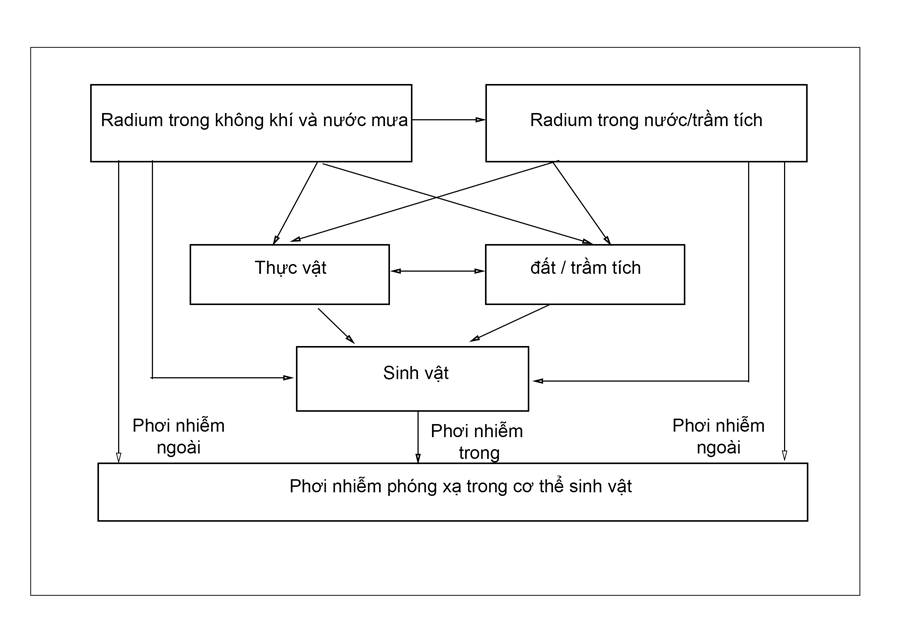
\includegraphics[width=0.95\textwidth]{Image/RadiumInBiota.png}
    \caption{Mô hình phát tán radium trong tự nhiên ~\cite{IAEANo476:revise}}
    \label{figure:RadiumToBiota}
\end{figure}
% TODO: --------------- Doc them tai lieu LAEA 410 -> Bo sung y nghia cua hinh RadiumToBioTa


   \subsection{Phân bố radium trong đất}

   Đất được hình thành từ quá trình phong hóa của đá mẹ dưới tác động của các yếu tố tự nhiên như: sự thay đổi nhiệt độ, độ ẩm, tác động của thời tiết, biến đổi khí hậu, tác động sinh học của động thực vật và con người. Do đó, các loại đất thường khác nhau về thuộc tính tùy thuộc vào đặc trưng của đá mẹ và các tác nhân ảnh hưởng từ tự nhiên. Trong quá trình phong hóa đá mẹ hình thành đất, radium được phân bố lại từ đá sang đất. Sự di chuyển của radium trong hạt đất chịu tác động rất nhiều bởi các yếu tố tự nhiên. Một phần radium được hòa tan trong nước ngầm, nước suối. Thông qua các chuỗi thức ăn, radium có thể tồn tại trong động thực vật. Phần còn lại bị lắng đọng dưới dạng phù sa, hoàng thổ hoặc hấp thụ trong đá hoặc đất ~\cite{IAEANo310:revise}. 

   Radium trong đất thể hiện các đặc điểm hóa học của một kim loại kiềm thổ. Radium hoạt động hóa học mạnh, ái lực cao. Các phản ứng trao đổi ion trong đất đóng vai trò quan trọng, ảnh hưởng đến quá trình di chuyển radium. Mỗi loại đất có các đặc tính khác nhau, khả năng trao đổi ion của các muối radium trong mỗi loại đất cũng khác nhau. Điều này ảnh hưởng đáng kể đến phân bố hàm lượng radium trong đất. Bảng ~\ref{table:RaDifferentofSoil} thể hiện hàm lượng \ce{^223Ra} trong một số loại đất khác nhau. Theo đó, hàm lượng \ce{^223Ra} trong đất dao động từ 3,7 đến 125,8 (Bq/kg). Đáng chú ý là đất nâu sa mạc ở CHLB Nga là loại đất có hàm lượng \ce{^226Ra} khá cao, từ 70,3 đến 125,8 (Bq/kg) \cite{IAEANo310:revise}.   
   
   \begin{table}[htbp]
        \centering
       \caption{Hàm lượng \ce{^226Ra} trong một số loại đất khác nhau ~\cite{IAEANo310:revise}}
       \begin{tabular}{ccc}
            \toprule
            Loại đất    &   Địa điểm    &   Hàm lượng \ce{^226Ra} (Bq/kg) \\
            \midrule
            Đất sét đỏ  & Florida, Hoa Kì  &   7,4\\
            Đất cát  &  Tây Ban Nha &  14,0 \\
            Đất Podzol  & CHLB Nga  & 33,3  \\
            Đất rừng xám  & CHLB Nga  & 37,1  \\
            Đất sét đen  & CHLB Nga  & 29,6  \\
            Đất rừng nâu  & CHLB Nga  & 29,6  \\
            Đất đỏ  & CHLB Nga  & 40,7  \\
            Đất xám/đất sa mạc  & CHLB Nga  & 18,5 \\
            Đất nâu sa mạc   & CHLB Nga  & 70,3 - 126  \\
            \bottomrule
        \end{tabular}
       \label{table:RaDifferentofSoil}
   \end{table}
   
        Bảng ~\ref{table:RaDifferentofCountry} thể hiện hàm lượng \ce{^226Ra} trong đất ở một số quốc gia khác nhau. Hàm lượng 226Ra nằm trong khoảng 2,59 - 140,6 (Bq/kg) đối với tất cả các quốc gia này.  ~\cite{IAEANo310:revise}.

    \begin{table}[htbp]
        \centering
        \caption{Hàm lượng \ce{^226Ra} trong đất ở một số quốc gia ~\cite{IAEANo310:revise}}
        \begin{tabular}{cc}
            \toprule
            Quốc gia   &   Hàm lượng \ce{^226Ra}  (Bq/kg)\\
            \midrule
            Tiệp Khắc   & 3,7 - 141\\
           Đức          & 13,0 - 48,1\\
            Ireland     & 48,1 - 107\\
            Anh         & 2,96 - 55,5\\
            CHLB Nga    & 3,7 - 48,1 \\
            Phần Lan    & 37 - 51,8\\
            Hoa Kì      & 29,6 - 104\\
            Nam Tư      & 29,4 - 37,4\\
            Nhật Bản    &  5,55 - 38,9\\
            Ấn Độ       & 2,59 - 26,3\\

            \bottomrule
        \end{tabular}
        \label{table:RaDifferentofCountry}
    \end{table}
 
    Bảng ~\ref{table:RaHighConcentration} thể hiện một số khu vực có hàm lượng \ce{^226Ra} cao nhất trên thế giới. Giá trị cao nhất đo được tại các vùng Ramsar, Iran và Cộng hòa Komi, CHLB Nga, vượt va so với hàm lượng \ce{^226Ra} trung bình trong đất trên thế giới theo tiêu chuẩn UNSCEAR  ~\cite{IAEANo476:revise}. 
    
    \begin{table}[htbp]
        \centering
        \caption{Hàm lượng \ce{^226Ra} trong đất ở một số khu vực cao nhất thế giới ~\cite{IAEANo476:revise}}
        \begin{tabular}{cc}
            \toprule
            Quốc gia    & Hàm lượng \ce{^226Ra} (Bq/kg) \\
            \midrule
            Kerala, Ấn Độ & 7,8-1520 \\
            Araxa, Brazil &  703-42400 \\
            Tapira, Brazil &  7814-28 800 \\
            Núi Ambazac Pháp &  950-8860 \\
            Ramsar, Iran  & 740-37 000 \\
            Niue, New Zealand & 6920-12 400 \\
            \bottomrule
        \end{tabular}
        \label{table:RaHighConcentration}
    \end{table}

    \subsection{Phân bố radium trong nước ngầm }
    

Radium trong nước ngầm là kết quả tương tác của dòng chảy mạch nước ngầm qua bề mặt, khe nứt của đá,... Các tương tác này tạo điều kiện cho radium sinh ra từ đồng vị mẹ dễ dàng hoà tan vào nước. Hàm lượng phóng xạ radium trong nước còn phụ thuộc mạnh vào các đặc điểm địa chất, độ sâu mực nước, độ pH, tốc độ dòng chảy, nhiệt độ môi trường nước, thời điểm lấy nước, và lượng mưa. Bên cạnh đó, các quá trình khai thác nhiên liệu, khai thác quặng uranium để sản xuất nguyên liệu hạt nhân, khai thác quặng photphat - apatit để sản xuất phân lân, vàng, than đá, ... cũng góp phần làm tăng đáng kể hàm lượng phóng xạ radium trong nước.

Với đặc tính dễ hòa tan của muối radium và tạo phức kết tủa với muối sulphat của barium va canxi, qua các khe nứt của thành đá gây ra bởi các hoạt động khai thác của con người, radium dễ dàng có mặt trong mạch nước. Quá trình khai thác dầu khí tạo ra một lượng lớn bùn thải. Việc xử lí bùn thải do khai thác dầu khí thường rất tốn kém nên đa phần được chôn lấp. Điều này dẫn đến nhiều rủi ro ô nhiễm phóng xạ, đặc biệt là mạch nước ngầm tại các khu vực dễ tiếp xúc với bùn thải ~\cite{IAEANo476:revise}.
 

Nồng độ \ce{^226Ra} trong nước ngầm tại một số khu vực trên thế giới được thể hiện trong bảng ~\ref{table:RadiumInGroundWater}. Theo đó, \ce{^226Ra} có nồng độ khá cao trong một số loại nước ở các khu vực khác nhau như khoáng nóng tại Nhật Bản (1300-7840 mBq/L), nước ngầm tại vùng khai thác uranium ở Texas - Hoa Kì (14,8-6290 mBq/L), nước nóng của địa nhiệt tại miền Tây - Hoa Kì (1,52-55 500) ~\cite{IAEANo476:revise}.

\begin{table}[htbp]
    \centering
    \caption{Nồng độ \ce{^226Ra} trong nước ngầm ở một số khu vực ~\cite{IAEANo476:revise}}
    \begin{tabular}{c c >{\centering\arraybackslash}m{3.7cm} c }
        \toprule
        Địa điểm    &   Nguồn nước &    Mô tả   & Nồng độ \ce{^226Ra} (mBq/L)\\
        \midrule
        Salzburg, Áo & Nước giếng &  & <3,7-270 \\
        Helsinki, Phần Lan & Nước giếng khoan &  & <3,7-9470 \\
      Pháp & Nước suối khoáng &  &163 \\
        Anh  & Nước khoáng nóng &  &374-525 \\
        \midrule
        Nhật Bản & Nước khoáng nóng  &  & 1300-7840\\
        Ả Rập Xê Út & Nước suối  &  & 699\\
        Đài Loan & Nước khoáng nóng  &  & 1,85-588\\
        \midrule
        Ottawa,Hoa Kì & Nước giếng & Nước đã lọc tại nhà máy & 3,7-570 \\
        Illinois,Hoa Kì & Nước giếng & Nước chưa qua xử lí & 0,74-836 \\
        Ottawa,Hoa Kì & Nước giếng & Nước đã lọc tại nhà máy & 3,7-570 \\
        Grants,Hoa Kì & Nước ngầm & Nhà máy khai thác quặng uranium & 1,9-1960 \\
        Texas,Hoa Kì & Nước ngầm & Nhà máy khai thác và nghiền quặng uranium & 14,8-6290 \\
        Florida,Hoa Kì & Nước ngầm & Nhà máy khai thác quặng photphat & 2810 \\
        Miền Tây, Hoa Kì & Nước nóng của địa nhiệt & Rò rĩ nguồn nước địa nhiệt & 1,52 - 55 550 \\
        \midrule 
        Yeelirrie, Úc & Nước ngầm & Mỏ quặng uranium & 18,5-33 400 \\
        \bottomrule
    \end{tabular}
    \label{table:RadiumInGroundWater}
\end{table}



\subsection{Phân bố radium trong không khí }

Bên cạnh tập trung trong đất và nước ngầm, một phần radium cũng tồn tại trong các hạt bụi khí nhỏ. Nồng độ \ce{^226Ra} trung bình trong bụi khí trên thế giới khoảng $1,5\mu Bq/m^3$ ~\cite{IAEANo476:revise}. Các hoạt động khai thác nhiên liệu của con người góp phần làm tăng nồng độ radium trong bụi khí. Đặc biệt, trong đó, ngành công nghiệp nhiệt điện là một trong những ngành làm tăng đáng kể nồng độ radium trong không khí. Trong quá trình đốt than, nhiệt độ lên đến $1700 ^\circ C$, than được nung nóng chảy thành tro. Tro bay cùng với hơi nước được thải ra ngoài khí quyển, đóng góp đáng kể vào lượng radium trong không khí. Bên cạnh đó, lượng tro bay này có thể lắng đọng xuống mặt đất, thảm thực vật hoặc nước mặt và thậm chí có thể xâm nhập vào nước ngầm.
            
\section{Ảnh hưởng của radium đến sức khỏe con người}

Thông qua nhiều chuỗi chuyển hóa sinh - hóa và chuỗi thức ăn mà radium có thể tồn tại trong cơ thể con người và sinh vật. Hình ~\ref{figure:RadiumToHuman} thể hiện tóm quá trình chuyển hóa radium từ môi trường tự nhiên vào cơ thể con người. Quá trình này diễn ra phức tạp và chịu ảnh hưởng bởi nhiều yếu tố trong môi trường và sinh vật. Về cơ bản, radium từ môi trường đi vào cơ thể con người chủ yếu qua đường hô hấp và tiêu hóa ~\cite{IAEANo476:revise}.

Trong cơ thể con người, radium phân rã alpha, hình thành các đồng vị con cháu phân rã alpha, beta hoặc gamma \cite{IAEANo310:revise}. Đồng vị \ce{^226Ra} là đồng vị phóng xạ nguy hiểm hơn cả do chu kỳ bán rã lớn, xác suất phát alpha cao, năng lượng phân rã lớn. Trong cơ thể con người, \ce{^226Ra} chủ yếu tích tụ trong xương, răng. Với khoảng 2,5 mg \ce{^226Ra} trong cơ thể, con người sẽ nhận một liều chiếu khoảng 25 Sv. Các bệnh thường gây ra khi chủ yếu tập trung ở xương, rrangnhư ung thư xương, thoái hóa xương, răng,...~\cite{Thesis:HNPThu}.

   \begin{figure}[htbp]
    \centering
    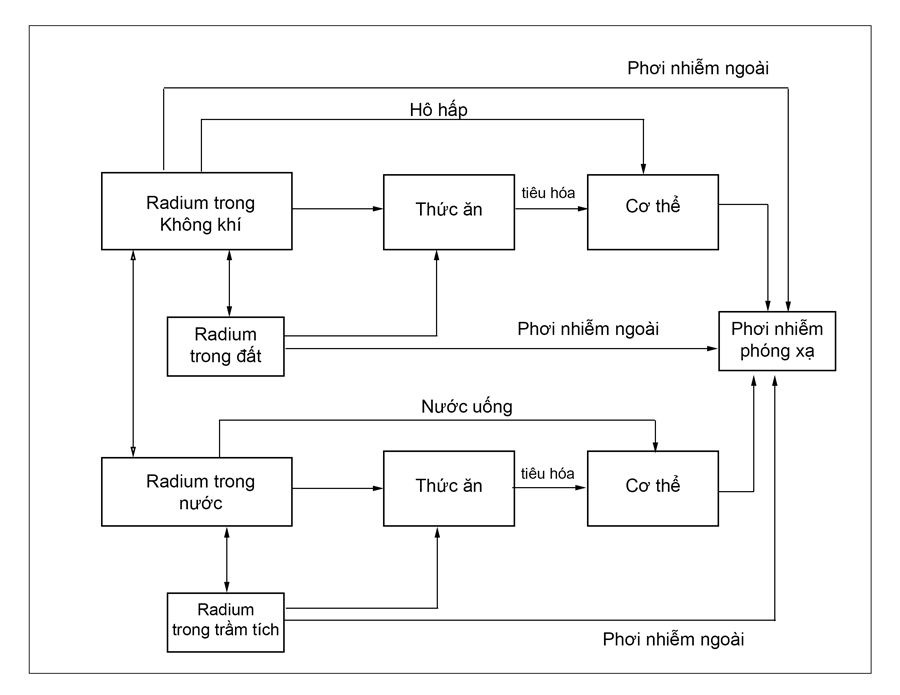
\includegraphics[width=0.75\textwidth]{Image/RadiumInHuman.png}
    \caption{Sơ đồ các con đường di chuyển của radium từ môi trường vào cơ thể người ~\cite{IAEANo476:revise}}
    \label{figure:RadiumToHuman}
\end{figure}
      
\clearpage



% ----------- Track Changes 
% REVIEW: 2019.01.06 - 11.51PM: Completed
% \setcounter{chapter}{1}
% Setting Chapter 2
%  
\chapter{Quy trình thực nghiệm lọc tách \ce{^226Ra} trong đất và nước}

\section{Đôi nét về  quy trình chiết tách/lọc \ce{^226Ra} trong đất và nước ngầm}

    \subsection{Quy trình chiết tách phân đoạn BCR}

    Những năm đầu 1990, các nghiên cứu về xây dựng quy trình chiết tách phân đoạn kim loại nặng, nổi bật như Koguh và cộng sự (1994), Kozuh  và cộng sự (1996), Ure và cộng sự (1996). Mục tiêu của quy trình nhằm đánh giá khả năng hòa tan trong nước trong từng pha, và tính linh động trong môi trường, từ đó có phương pháp cụ thể để loại bỏ các kim loại nặng trong đất và trầm tích ~\cite{BCR:OrginNusa}. Mỗi quy trình lại tập trung cụ thể vào một kim loại, và hóa chất phân tích được lựa chọn có độ hoạt động hóa học cao với kim loại phân tích đó. Do đó, dữ liệu thu được của mỗi nghiên cứu không thể được so sánh, hoặc tham khảo. Năm 1987, nhằm xây dựng một quy trình chiết tách kim loại có tính tiêu chuẩn và đồng bộ, một nhóm các chuyên gia của Viện tiêu chuẩn và đo lường Châu Âu \footnote{Institute for Reference Materials and Measurements: Viện được thành lập vào năm 1957 theo Hiệp ước Rome và bắt đầu hoạt động vào năm 1960 dưới tên của Cục tiêu chuẩn đo lường Hạt nhân (CBNM). Năm 1986, Viện đổi tên thành Ủy ban về đo lường Châu Âu. Năm 1993, Viện chính thức đổi tên là Viện tiêu chuẩn về đo lường Châu Âu, tập trung về xây dựng tiêu chuẩn đo lường từ an toàn thực phẩm đến ô nhiễm môi trường, có trụ sở chính đặt tại Bỉ (Theo en.wikipedia.org)} đã đề xuất một quy trình trích xuất ba bước (BCR CRM - 601), từ dữ liệu thu được có thể xác định độ linh động của kim loại nặng  trong từng phân đoạn. ~\cite{BCR:PeterSvete}.  Quy trình BCR được áp dụng rộng rãi trong phân tích kim loại nặng trong đất, bùn, và trầm tích. Ưu điểm của quy trình, là sự thống nhất trong phân tích các kim loại nặng, và sử dụng mẫu chuẩn để phân tích, kết quả phân tích được chứng nhận tiêu chuẩn Châu Âu, và giảm thời gian phân tích. Quy trình BCR CRM-601 gồm ba phân đoạn chính:
        \begin{enumerate}[label=(\arabic*) ]
            \item Phân đoạn trao đổi ion và axit hóa: Trao đổi ion kim loại và liên kết với cacbonat.
            \item Phân đoạn khử: Liên kết của Sắt and mangan hydroxide
            \item Phân đoạn oxi-hóa: Liên kết hữu cơ và sulfua
        \end{enumerate}


    \subsection{Phương pháp hấp thụ \ce{^226Ra} bằng sợi \ce{MnO2}}

      Từ nghiên cứu của nhóm  Willard S. Moore (1973) về các đặc tính thuỷ văn hải dương như: quỹ đạo vận chuyển của khối nước biển ven bờ, sự pha trộn theo chiều đứng và chiều ngang của nước gần bờ với nước đại dương, tốc độ bổ cấp nước ngầm... sử dụng  hai đồng vị có thời gian bán rã dài là \ce{^226Ra} và \ce{^228Ra} có sử dụng làm  đồng vị đánh dấu và chỉ thị môi trường ~\cite{MnO2:Moore} . Trong quá trình nghiên cứu, nhóm đã xây dựng và phát triển phương pháp hấp thụ \ce{^226Ra} trong nước bằng sợi acrylic tẩm mangan oxit.
      
      Các kết quả phân tích , nhóm Willard S. Moore đã nhận xét rằng: 
      \begin{itemize}
        \item Phương pháp đồng kết tủa radium với \ce{BaSO4}, không phù hợp để tạo sợi lọc nước biển. 
        \item \ce{MnO2/Mn(OH)2} hấp thụ \ce{^226Ra} tốt so với sắt oxit của nhóm nhóm Krishnaswami (1972). Cụ thể, phương pháp lọc bằng sợi mangan oxit có hiệu suất lọc \ce{^226Ra} trên 90\% từ 170L nước biển, với tốc độ dòng chảy 400 cm/phút, trong khi sợi Sắt oxit chỉ có hiệu suất lọc khoảng 11\%.
        \item  Nhóm đã đề xuất cải tiến phương pháp bằng tẩm sợi acrylic với các muối \ce{MnCO3}, \ce{FeS}, và \ce{MnS}, có thể tăng hiệu suất lọc radium. Bên cạnh đó, muối Zirconium (\ce{[OH]^-}, \ce{[PO4] ^{3-}} và   \ce{[Mo4]^{2-}}) có hiệu suất hấp thụ radium cao nhất, nhưng chi phí của Zirconium khá cao, không phù hợp để lọc thể tích mẫu nước biển (từ 1L trở lên). 
    \end{itemize}
    
    Dựa trên thành công của phương pháp lọc \ce{^226Ra} bằng sợi acrylic tẩm \ce{MnO2} của nhóm Willard S. Moore (1973), tác giả  cải tiến  phương pháp sử dụng sợi tổng hợp tẩm   \ce{MnO2} thay vì sử dụng sợi acrylic tẩm \ce{MnO2}. 




    % TODO: --------------------------------------------------------------------

\section{Hệ thiết bị RAD7}
\label{section:HeThietBiRAD7}

Hệ thiết bị  RAD7,  là thiết bị chuyên sử dụng để đo khí \ce{^222Rn} và \ce{^220Rn} hoàn chỉnh, đáp ứng nhiều mục đích sử dụng khác nhau. Hệ thiết bị RA7 đi kèm các phụ kiện như ~\cite{Thesis:HNPThu}: 
    \begin{itemize}
        \item Các lọ chứa    mẫu nước đo dung tích 250 mL và 40 mL.
        \item Bộ phận thu khí radon trong nước gồm: khối ba đầu làm bằng kim loại
        không gỉ, ống nhựa đôi dùng để giữ khối ba đầu, ống đệm bằng vật liệu tổng hợp, đầu sục khí.
        \item Ống chứa than hoạt tính.
        \item Các đầu lọc khí và ống dẫn khí từ ngoài vào RAD7 và từ RAD7 ra ngoài.
    \end{itemize} 
    


    Sơ đồ hệ thí nghiệm đo nồng độ radon để xác định hàm lượng \ce{^226Ra} đã lọc tách chứa trong phần mẫu lỏng  được thể hiện trên hình ~\ref{figure:SoDoLayRnRD7}. Khi bắt đầu quá trình đo, bơm trong RAD7 sục khí vào lọ đựng mẫu, đẩy khí phóng xạ hòa tan trong lọ ra khỏi nước và tạo thành dòng lưu thông khép kín đi qua buồng đo. Hiệu suất tách radon khỏi nước, đưa vào vòng không khí khoảng 94\% đối với lọ 250 ml. Radon thoát khỏi mẫu nước, liên tục tuần hoàn qua ống hút ẩm, buồng đo và sau đó trở về mẫu nước để thiết lập trạng thái cân bằng giữa radon trong nước và không khí. Sau 5 phút, bơm trong RAD7 sẽ dừng hoạt động. Ngắt kết nối giữa mẫu và RAD7, hệ thiết bị được đóng kín và hoạt động đo trong 4 đến 5 giờ. 


    
    \begin{figure}[htbp]
        \centering
        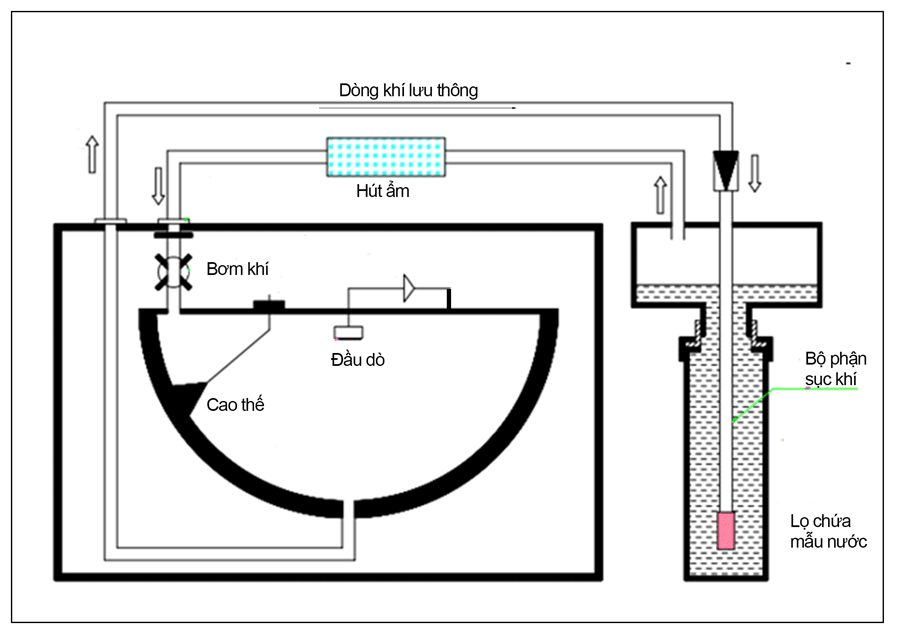
\includegraphics[width=0.75\textwidth]{Image/MnO2-Figure7.png}
        \caption{Sơ đồ lấy khí radon trong mẫu nước và đo bằng RAD7}
        \label{figure:SoDoLayRnRD7}
    \end{figure}



    \textbf{Nguyên lý xác định nồng độ radon của RAD7} ~\cite{Thesis:HNPThu}: 
    
    Buồng đo khí phóng xạ bên trong RAD7 có hình bán cầu, được phủ phía trong một lớp dẫn điện. Bộ phận ghi nhận tín hiệu làm bằng tấm silicon phẳng và được đặt ở tâm bán cầu. Mạch điện cung cấp điện áp (2000 - 2500) V, tạo nên điện trường trong toàn bộ buồng đo. Điện trường giúp đẩy các hạt tích điện đến đầu dò. RAD7 xác định nồng độ radon dựa vào việc đo phổ năng lượng của tia alpha. Khi bắt đầu quá trình đo, máy bơm đưa khí chứa radon (đã được làm khô) vào buồng. Đầu lọc khí chỉ cho khí hiếm đi qua và ngăn cản các đồng vị con cháu gây ảnh hưởng đến kết quả đo. Radon là nguyên tử khí trung hòa về điện nên không được hệ đo ghi nhận cho đến khi phân rã, tạo thành \ce{^218Po}, tồn tại dạng ion dương. Điện trường trong buồng đo mang các hạt tích điện dương đến đầu dò. \ce{^218Po} phân rã ngay trên bề mặt đầu dò. Hạt alpha tạo ra có khả năng đập vào đầu dò và tạo nên xung điện có độ lớn tỷ lệ thuận với năng lượng. Các quá trình phân rã tiếp tục diễn ra tạo thành các hạt alpha có năng lượng khác nhau, sinh ra các tín hiệu có biên độ khác nhau, được khuếch đại và chuyển thành tín hiệu số nhờ các mạch điện. Bộ xử lý thu nhận các tín hiệu, lưu trữ trong bộ nhớ theo năng lượng của từng hạt alpha và xây dựng các đỉnh phổ năng lượng riêng biệt. Số đếm ở các cửa sổ A (\ce{^218Po}) và C (\ce{^214Po}) để xác định nồng độ radon vì chúng ghi nhận alpha từ phân rã của các con cháu radon. Số đếm ở các cửa số B (\ce{^216Po}) và D (\ce{^212Po}) được ghi nhận để xác định nồng độ thoron vì chúng chứa số đếm từ các con cháu của thoron. Hình ~\ref{figure:PhoAlphaRAD7} minh họa ví dụ một phổ alpha lấy từ RAD7. Thông thường, khoảng sau 3 giờ, số đếm ở cửa sổ C sẽ cân bằng với số đếm ở cửa sổ A. Vì vậy, 3 giờ đầu, nồng độ radon sẽ được xác định dựa vào số đếm ở cửa sổ A, sau đó, cả số đếm ở cửa sổ A và cửa sổ C đều được dùng để xác định nồng độ radon . Ngoài ra, RAD7 gộp các tín hiệu nhiễu và số đếm alpha ghi nhận được từ đồng vị \ce{^210Po} vào cửa sổ O. \ce{^210Po} là đồng vị con cháu của radon xuất hiện khi máy được sử dụng trong một thời gian dài. Các số đếm này không đóng góp vào nồng độ radon vì đã được đưa vào một cửa sổ khác. Đây là điểm ưu việt của RAD7.


    \begin{figure}[htbp]
        \centering
        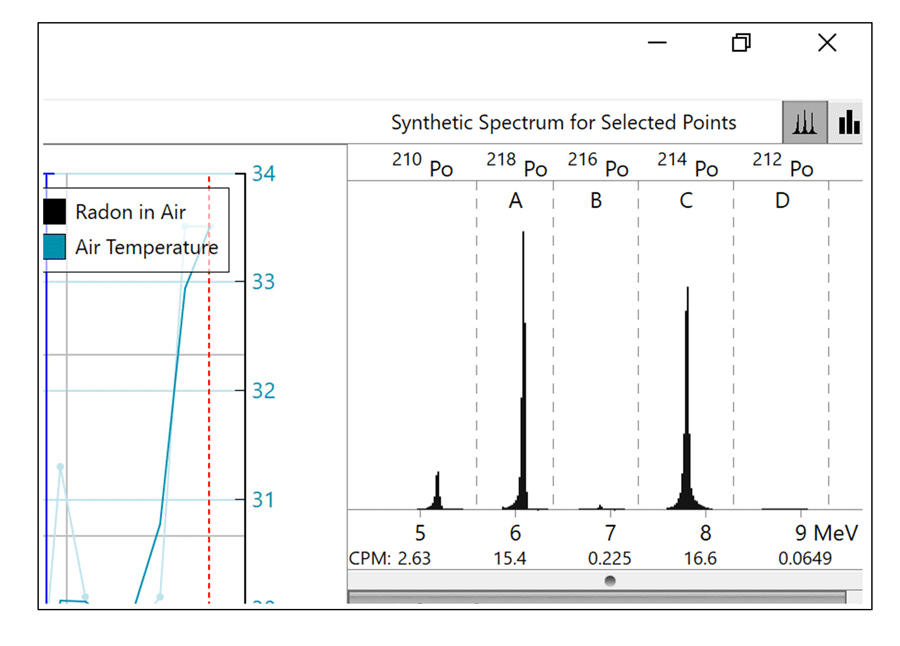
\includegraphics[width=0.68\textwidth]{Image/MnO2-Figure2.png}
        \caption{Phổ alpha lấy từ RAD7}
        \label{figure:PhoAlphaRAD7}
    \end{figure}
    

    \textbf{Đo nồng độ \ce{^222Rn} trong mẫu nước bằng hệ thiết bị RAD7}

\begin{itemize}
    \item Trên màn hình hiển thị của RAD7, chọn mục Setup thiết lập các chế độ đo.
    \item Tại cửa Inlet, ta thực hiện nối máy với ống hút ẩm qua đầu lọc và dây dẫn khí,  đầu còn lại của ống được nối vào bộ phận thu khí từ lọ nước.
    \item Tại cửa Outlet của RAD7, ta thực hiện nối bộ phận thu khí từ lọ nước.
    \item Để tiến hành đo, ta thực hiện: chọn Test, chọn Start và chọn Enter để bắt đầu quá trình đo.
    \item Khi hết thời gian đo, máy sẽ tự động dừng. Trong trường hợp gặp phải sự cố, để dừng đo tức thời, ta thực hiện, chọn Test, rồi chọn Stop 
    \item Làm sạch máy.
    \item Lấy số liệu: Khi đo xong, kết quả có thể được xuất ra máy in hoặc chuyển sang máy tính
    nhờ dây cáp nối máy tính - RAD7 và phần mềm CAPTURE.
\end{itemize}

 
    % FIX Lai hinh DigramRAD7
    \begin{figure}[htbp]
        \centering 
        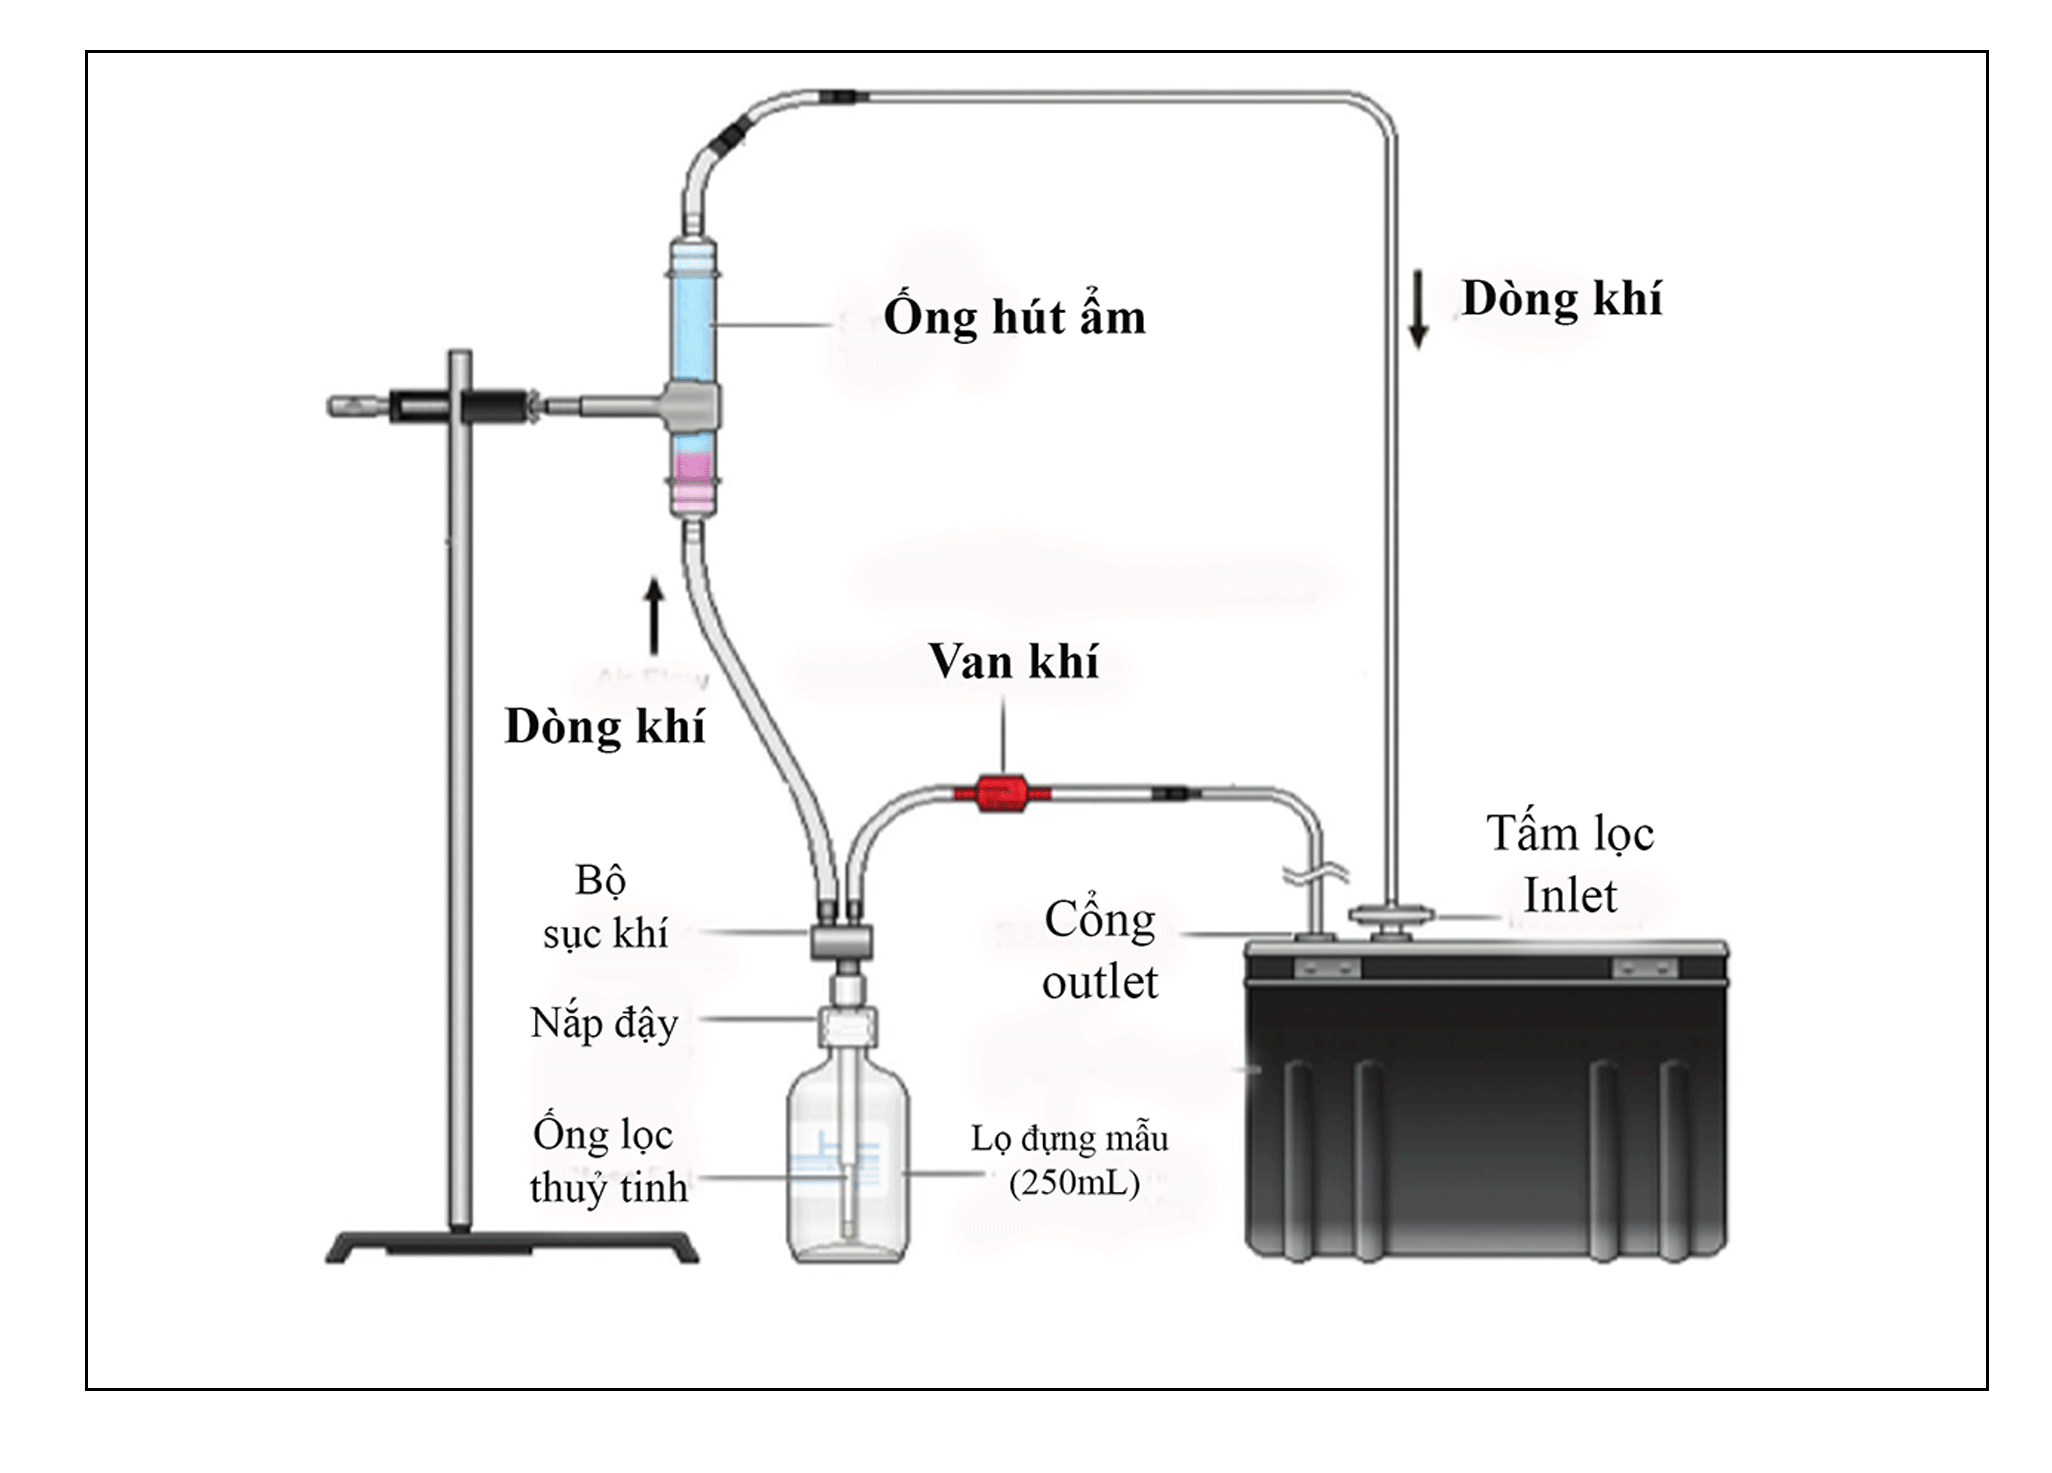
\includegraphics[width=0.75\textwidth]{Image/MnO2-Figure1.png}
        \caption{Sơ đồ bố trí đo khí \ce{^222Rn} của mẫu nước bằng hệ thiết bị RAD7}
        \label{figure:RADSoDoDoMauNuoc}
    \end{figure}



        % TODO: BCR ------------------------------------------
        \subsection{Xác định nồng độ \ce{^226Ra} chiết tách được sau mỗi phân đoạn của  quy trình BCR}
    Mẫu nước được tách ra sau khi li tâm ở mỗi phân đoạn được nhốt trong vòng 10 ngày. Trong thời gian này,  \ce{^226Ra} tồn tại trong nước phân rã alpha đồng vị \ce{^222Rn}. Khi lượng \ce{^222Rn} sinh ra đủ lớn, ta tiến hành đo nồng độ \ce{^222Rn} trong nước bằng thiết bị RAD7.    Hàm lượng \ce{^226Ra} trong phần lỏng thu được qua mỗi bước chiết tách được xác định gián tiếp thông qua nồng độ \ce{^222Rn} theo công thức ~\ref{equationBCR:RntoRa}: 
    
    \begin{equation}
        C_{Ra} = \dfrac{k.C_{Rn}.V}{\qty(1-e^{-\lambda.t})m}
        \label{equationBCR:RntoRa}
    \end{equation}
    
    
    Sai số kết quả được xác định theo công thức ~\ref{equationBCR:SigmaRntoRa}. 
    \begin{equation}
        \sigma_{C_{Ra}} = C_{Ra}.\sqrt{\qty(\dfrac{\sigma_{Rn}}{C_{Rn}})^2 + \qty(\dfrac{\sigma_{k}}{k})^2 }
        \label{equationBCR:SigmaRntoRa}
    \end{equation}
    
    
    Trong đó:
    \begin{itemize}
    \item  $C_{Rn} \pm \sigma_{C_{Rn}}$  (Bq/L) là nồng độ phóng xạ của \ce{^222Rn} trong 250 ml dung dịch mẫu và sai số;  V = 250 (mL) là thể tích dung dịch mẫu; Khối lượng mẫu đất đem phân tích, m = 10 g.
    \item $C_{Ra} \pm \sigma_{C_{Ra}}$ (Bq/kg) là nồng độ phóng xạ của \ce{^226Ra} trong phần lỏng sau khi lọc tách trong mỗi bước của mẫu cần phân tích và sai số;
    \item Thời gian nhốt t = 10 ngày; Hằng số phân rã của \ce{^222Rn} = $0.2621 (\text{ngày}^{-1})$
    \item Hệ số k là hệ số hiệu chỉnh sự thất thoát radon trong quá trình nhốt mẫu. Hệ số k được xác định bằng cách sử dụng nguồn chuẩn \ce{^226Ra} hoạt độ xấp xỉ 5 Bq của NIST. Nguồn được nhốt 10 ngày trong lọ chuyên dụng của RAD7 chứa 250 ml nước cất. Hệ số k là tỷ số giữa hoạt độ được cung cấp bởi nhà sản xuất và hoạt độ đo được bằng RAD7. Hệ số k được xác định trung bình qua 5 lần nhốt mẫu và đo. Hệ số trung bình đạt $1,25 \pm 0,03$ ~\cite{Thesis:HNPThu}. 
    
    \end{itemize}
    
    % TODO: ------------------------ MnO2


    \subsection{Xác định nồng độ \ce{^226Ra} trước và sau khi thực hiện phương pháp hấp thụ \ce{MnO2}}

    Mẫu nước trước và sau khi lọc tách bằng phương pháp hấp thụ \ce{^226Ra} trên sợi tổng hợp, sẽ được nhốt trong lọ kín 250 ml trong 10 ngày. Sau đó, nồng độ \ce{^226Ra} được xác định bằng hệ thiết bị RAD7,  từ công thức (~\ref{equation:RntoRa}), ta có thể suy ra nồng độ \ce{^226Ra}  trong mẫu nước.

        \begin{equation}
            C_{Ra} = \dfrac{k.C_{Rn}}{\qty(1-e^{-\lambda.t})}
            \label{equation:RntoRa}
        \end{equation}

        \begin{equation}
            \sigma_{Ra} = C_{Ra}.\sqrt{\qty(\dfrac{\sigma_{Rn}}{C_{Rn}})^2 + \qty(\dfrac{\sigma_{k}}{k})^2 }
        \end{equation}

Trong đó:
\begin{itemize}
    \item  $C_{Rn} \pm \sigma_{C_{Rn}}$  (Bq/L) là nồng độ phóng xạ của \ce{^222Rn} trong 250 ml dung dịch mẫu;  V = 250 (mL)
    \item $C_{Ra} \pm \sigma_{C_{Ra}}$ (Bq/L) là nồng độ phóng xạ của \ce{^226Ra} trong phần lỏng sau khi lọc tách  của mẫu cần phân tích;
    \item Thời gian nhốt t = 10 ngày; Hằng số phân rã của \ce{^222Rn} = $0.2621 (\text{ngày}^{-1})$
    \item Hệ số k là hệ số hiệu chỉnh sự thất thoát radon trong quá trình nhốt mẫu. Hệ số k được xác định bằng cách sử dụng nguồn chuẩn \ce{^226Ra} hoạt độ xấp xỉ 5 Bq của NIST. Nguồn được nhốt 10 ngày trong lọ chuyên dụng của RAD7 chứa 250 ml nước cất. Hệ số k là tỷ số giữa hoạt độ được cung cấp bởi nhà sản xuất và hoạt độ đo được bằng RAD7. Hệ số k được xác định trung bình qua 5 lần nhốt mẫu và đo. Hệ số trung bình đạt $1,25 \pm 0,03$ ~\cite{Thesis:HNPThu}. 
    
\end{itemize}

    

\section{ Quy trình thực nghiệm lọc tách \ce{^226Ra} trong đất}
Quy trình lọc tách \ce{^226Ra} được áp dụng trên một số mẫu đất được thu thập tại khu vực Ninh Sơn, tỉnh Ninh Thuận. Khu vực này có một số mẫu đất chứa hàm lượng phóng xạ \ce{^226Ra} cao trên mức trung bình trên thế giới theo UNSCEAR (Thu, 2019).

%    FIXME: Thu,2019 là gì


\subsection{Xác định hàm lượng \ce{^226Ra} trong đất}

    \textbf{Chuẩn bị mẫu đất} 

    \begin{itemize}
        \item Mẫu đất tại hiện trường được lấy ở độ sâu từ 20 – 30 cm. Sau khi được di chuyển về phòng thí nghiệm, mẫu được hong khô, nhặt sạch các dị vật: sỏi đá, rác. 
        \item   Mẫu đất khô được nghiền nhỏ, rây qua rây có đường kính lỗ 0,2 mm để đảm bảo mẫu được đồng nhất. Tiếp tục sấy mẫu ở nhiệt độ 105 (độ C) trong 8 (giờ) và đóng mẫu vào hộp trụ. Lưu ý mẫu cần được đóng đồng đều, chiều cao khoảng 2 cm, đảm bảo độ kín của hộp tốt nhất có thể.
        \item  Nhốt mẫu ít nhất 30 ngày để tạo cân bằng phóng xạ giữa \ce{^226Ra} và các đồng vị con cháu trước khi đo bằng hệ phổ kế gamma.
    \end{itemize}



    
    \textbf{Xác định hàm lượng \ce{^226Ra} bằng hệ phổ kế gamma}
   
    Hệ thiết bị được sử dụng để phân tích hàm lượng phóng xạ \ce{^226Ra} trong khóa luận là phổ kế gamma GC3520 của hãng Canberra, đặt tại Phòng thí nghiệm Kỹ thuật Hạt nhân. Hệ đo được thiết lập để ghi nhận bức xạ gamma với khoảng năng lượng từ 40 keV đến 3 MeV. 

    Hệ đo gồm các thiết bị: đầu dò và nguồn nuôi cao thế cho đầu dò, bộ phận khuếch đại và tiền khuếch đại, bộ phân tích đa kênh, buồng chì che chắn phông bao quanh đầu dò và nguồn, thiết bị làm lạnh cho đầu dò. Đầu dò HPGe có độ phân giải năng lượng và hiệu suất ghi tương đối tại đỉnh phổ có năng lượng 1332 keV của đồng vị \ce{^60Co} tương ứng là khoảng 1,95 keV và 40\%. Phần mềm được sử dụng để điều khiển hệ đo và phân tích phổ là Genie 2000. Hiệu suất được tính toán dựa vào mẫu chuẩn bằng phần mềm Angle.

    Hàm lượng \ce{^226Ra} được xác định thông qua các đỉnh năng lượng của các đồng vị con cháu. Các đồng vị dùng để xác định hàm lượng \ce{^226Ra} gồm \ce{^214Bi} (609,3 keV, 1120,3 keV, 1238,1 keV, 1764,5 keV) và \ce{^214Pb} (295,2 keV, 351,9 keV). Hàm lượng phóng xạ ứng với một đỉnh gamma được xác định theo công thức ~\ref{equation:CRaHPGe}

        \begin{equation}    
            A = \dfrac{N}{\varepsilon.I_\gamma.t.m}
            \label{equation:CRaHPGe}
        \end{equation}  

Trong đó, A (Bq/kg) là nồng độ hoạt độ của đồng vị quan tâm; N (số đếm) là diện tích đỉnh phổ đã trừ phông và hiệu chỉnh thời gian chết; m (g) là khối lượng mẫu đo, t (s) là thời gian đo; $\varepsilon$ và $I_\gamma$ lần lượt là hiệu suất tuyệt đối của đầu dò và xác suất phát của đỉnh gamma quan tâm.

    Sai số hoạt độ được xác định theo công thức ~\ref{equation:SigmaCRaHPGe}. 
        \begin{equation}
            \qty(\dfrac{\sigma_A}{A})^2 =  \qty(\dfrac{\sigma_N}{N})^2 + \qty(\dfrac{\sigma_m}{m})^2  + \qty(\dfrac{\sigma_t}{t})^2 + \qty(\dfrac{\sigma_I}{I})^2 + \qty(\dfrac{\sigma_\varepsilon}{\varepsilon})^2 
            \label{equation:SigmaCRaHPGe}
        \end{equation}

\subsection{ Quy trình chiết tách \ce{^226Ra} trong mẫu đất}

    \subsubsection{Thiết bị, dụng cụ và hóa chất}
    \textbf{Thiết bị}
        \begin{itemize}
            \item Hệ thiết bị RAD7 của hãng Durridge, Mỹ.
            \item Máy li tâm loại PLC series, mã số 1804790 của hãng Gemmy, Đài Loan.
            \item Máy lắc sang mẫu đất SKL-330, mã số TBTN01013.
            \item Cân điện tử tiểu li: Cân 5 số model PR227/E(2018) của công ty OHAUS, Mỹ (Khối lượng phân tích tối đa 200g, độ chính xác 0,01 mg).
            \item Đèn sấy hồng ngoại của Công ty NTE, Việt Nam (2018), công suất 250W
            \item Bút đo pH điện tử pHTestr30 Waterproof của Công ty OAKTON, Mỹ, giai đo từ –1.00 - 15.00 pH, ở nhiệt độ $0 - 50 ^\circ C$.
            
        \end{itemize}
    \textbf{Dụng cụ và vật liệu}
        \begin{itemize}
            \item Nhiệt kế thủy ngân ($0-100 ^\circ C$, sai số $0.1 ^\circ C$)
            \item Đũa thủy tinh (20cm) và muỗng nhôm.
            \item Cốc thủy tinh chia vạch (50mL, 200mL, 400mL và 500mL), pipet (2mL), micropipet các  loại của hãng DURAN, Đức.
            \item Lọ thủy tinh (250mL, độ chia nhỏ nhất 50mL) của hãng DURAN, Đức.
            \item Giấy lọc Whatman loại 1 (11 micron) của hãng Whatman, Mỹ.
        \end{itemize}
    \textbf{Hóa chất}
        \begin{itemize}
            \item Dung dịch \ce{HNO3} (65\%-300mL), \ce{HCl} (36,5\%-300mL), hydroperoxit (80\%-300mL), axit acetic \ce{CH3COOH} (90\% - 1,5L)  và dung dịch \ce{NH4OH} (30\%-300mL) của hãng Merck, Mỹ.
            \item Bột hydroxylamine hydrochloride \ce{HONH2HCl} (98,5\%), khối lượng 25 g của Công ty Xilleng Scientific, Đài Loan.
            \item Bột ammonium acetate (98,5\% ), khối lượng 500 g của Xilong Chemical, Trung Quốc. 
        \end{itemize}

        
    \subsubsection{Quy trình thực hiện}

        \textbf{Chuẩn bị dung dịch và mẫu đất}
        \begin{itemize}
            \item Mẫu đất được phơi khô bằng bếp điện trong nhiệt độ $150^\circ C$ trong vòng 3h, sau đố thực hiện cân 10 (g) mẫu đất bằng cân tiểu li.
            \item Ống nghiệm và lọ đựng phải đựng rửa sạch và tráng bằng dung dịch cồn (90 độ) để hạn chế bụi bẩn và nấm móc.
            \item  Dung dịch axit acetic (0.11M-400mL): dùng pipet lấy khoảng 2.64mL dung dịch axit acetic (16.9M) hòa tan trong 400mL.
            \item  Dung dịch hydroxylamine hydrochloride (0.1M-400mL): thu được bằng cách lấy 2.82g bột hydroxylamine hydrochloride hoa tan với nước cất 390mL.
            \item  Dung dịch ammonium acetate  (1M-500mL): thu được bằng cách lấy 39.2g bột ammonium acetate hoà tan với nước cất 480mL.
        \end{itemize}


        \textbf{Bước 1}: Phân đoạn trao đổi ion và axit hóa
        
        Lấy 10(g) mẫu đất có kích thước hạt nhỏ hơn 0,045 mm với 400 mL dung dịch axid acetic 0,11M, điều chỉnh pH = 2,8 bằng dung dịch axit \ce{HNO3} và \ce{NH4OH} loãng. Hỗn hợp gồm đất và axid acetic đựng trong bình thủy tinh đậy nắp kín. Hỗn hợp được lắc trộn đều với tốc độ 250 (vòng/phút) ở nhiệt độ 30 (độ C) trong 16 giờ bằng máy lắc SKL-330. Sau đó, mẫu chứa đất và dung dịch axid acetic được li tâm bằng máy li tâm để chia thành hai phần, phần rắn và phần lỏng. Phần rắn được rửa lại bằng nước cất để loại bỏ lượng axid còn tồn đọng. Phần dung dịch được nhốt kín trong 10 ngày để xác định hàm lượng \ce{^226Ra} đã được tách ra trong bước này.        

        \textbf{Bước 2}: Phân đoạn khử
        
        Cho vào phần rắn sau bước 1 hoà tan 400 mL dung dịch hydroxylamine hydrochloride 0.1M, điều chỉnh pH = 2 bằng dung dịch axit \ce{HNO3} và \ce{NH4OH} loãng. Hỗn hợp được lắc đều trong 16 giờ tương tự như trong bước 1. Phần rắn và phần lỏng được tách riêng biệt bằng máy li tâm. Phần rắn được rửa sạch bằng nước cất. Phần dung dịch được nhốt kín để xác định hàm lượng \ce{^226Ra} đã được tách ra trong bước này. 
        
                
        \textbf{Bước 3}: Phân đoạn oxi-hóa
        
        Thêm 100 mL dung dịch hydroperoxid 8,8M vào phần mẫu rắn ở bước 2. Hỗn hợp mẫu được lắc đều trong 1 giờ ở nhiệt độ phòng. Sau đó, mẫu được đun nóng ở nhiệt độ khoảng 85 (độ C) trong 1 giờ. Tiếp tục thêm 100 mL dung dịch hydroperoxide 8,8M và đun nóng hỗn hợp trong 1 giờ ở nhiệt độ 85 (độ C). Phần đất được để nguội, sau đó thêm vào 500mL amonium axetate 1M. Điều chỉnh pH = 2 bằng dung dịch \ce{HNO3} và \ce{NH4OH} loãng. Mẫu được lắc đều trong 16 giờ tương tự các bước 1 và 2. Phần rắn đất và phần lỏng được tách riêng biệt bằng máy li tâm. Phần rắn được rửa sạch bằng nước cất, rồi phơi khô bằng bếp điện ở nhiệt độ 105 (độ C), cuối cùng được đóng vào bao nilong. Phần mẫu lỏng được nhốt kín để xác định hàm lượng \ce{^226Ra} đã được tách ra trong bước này.
 

         Quy trình tách chiết \ce{^226Ra} ra khỏi mẫu đất có thể được trình bày ngắn gọn trong sơ đồ trong bảng ~\ref{table:BCRCM601}. 

    \begin{table}[ht]
        \centering
        \caption{Quy trình chiết tách phân đoạn liên tục BCR tách \ce{^226Ra} trong đất} %BA140
        \label{table:BCRCM601}
        \begin{tabularx}{\textwidth}{>{\centering\arraybackslash}p{1cm} >{\centering\arraybackslash}p{3.5cm} >{\centering\arraybackslash}p{4.0cm} >{\centering\arraybackslash}p{5.5cm}}
            \toprule
            Bước    & Phân đoạn & Pha     &      Mô tả\\
            \midrule
            1       &  Trao đổi ion, hòa tan trong nước và axit         &  Liên kết với cacbonat, trao đổi ion kim loại         &    (400mL - 0.11) M axit acetic       \\
            2       &  Khử         &  Sắt và mangan hydroxide       &  0.11M hydroxylammonium clorua pH=2      \\
            3       &  Oxi hóa     &   Liên kết hữu cơ và sulfua        &   8.8M Hydro peroxid +  1.0 M amoni axetat, pH=2     \\
            \bottomrule
        \end{tabularx}
    \end{table}


  
\subsubsection{Phân tích nồng độ \ce{^226Ra} sau khi chiết tách được trong từng phân đoạn}
  
Các mẫu lỏng chứa \ce{^226Ra} tách ra từ mỗi phân đoạn được nhốt trong vòng 10 ngày. Nồng độ \ce{^226Ra} được xác định thông qua đồng vị \ce{^222Rn} đo trên hệ thiết bị RAD7, như đã trình bày chi tiết ở mục ~\ref{section:HeThietBiRAD7}. 

\textbf{Hiệu suất lọc tách \ce{^226Ra} trong mẫu đất} 

Hiệu suất lọc tách \ce{^226Ra}, E (\%), trong mẫu đất qua mỗi bước được xác định theo công thức ~\ref{equation:E_BCR}
\begin{equation}
    E (\%) =  \dfrac{C_{ex}}{C_0}.100\% 
    \label{equation:E_BCR}
\end{equation} 

Sai số kết quả được xác định theo công thức ~\ref{equation:SigmaE_BCR}:
    \begin{equation}
        \dfrac{\sigma_E}{E} = \sqrt{\qty(\dfrac{\sigma_{C_0}}{C_0})^2  + \qty(\dfrac{\sigma_{C_{ex}}}{C_{ex}})^2   } 
        \label{equation:SigmaE_BCR} 
    \end{equation}

    Trong đó, $C_0 \pm \sigma_{C_0}$ (Bq/kg) là hàm lượng phóng xạ trong mẫu đất trước khi lọc tách và sai số; $C_{ex} \pm \sigma_{C_{ex}}$ (Bq/kg) là hàm lượng \ce{^226Ra} lọc tách được trong từng phân đoạn.
    Hiệu suất toàn bộ quy trình lọc tách \ce{^226Ra} trong đất được tính tổng lại từ hiệu suất thu được trong ba bước trên.
    

    
    


   Hình ~\ref{figure:DiagramRadiuminSoilBCR}, mô tả tóm tắt quy trình xử lí nhiễm bẩn \ce{^226Ra} trong đất bằng quy trình chiết tách phân đoạn BCR.

    \begin{figure}[htbp]
        \centering
        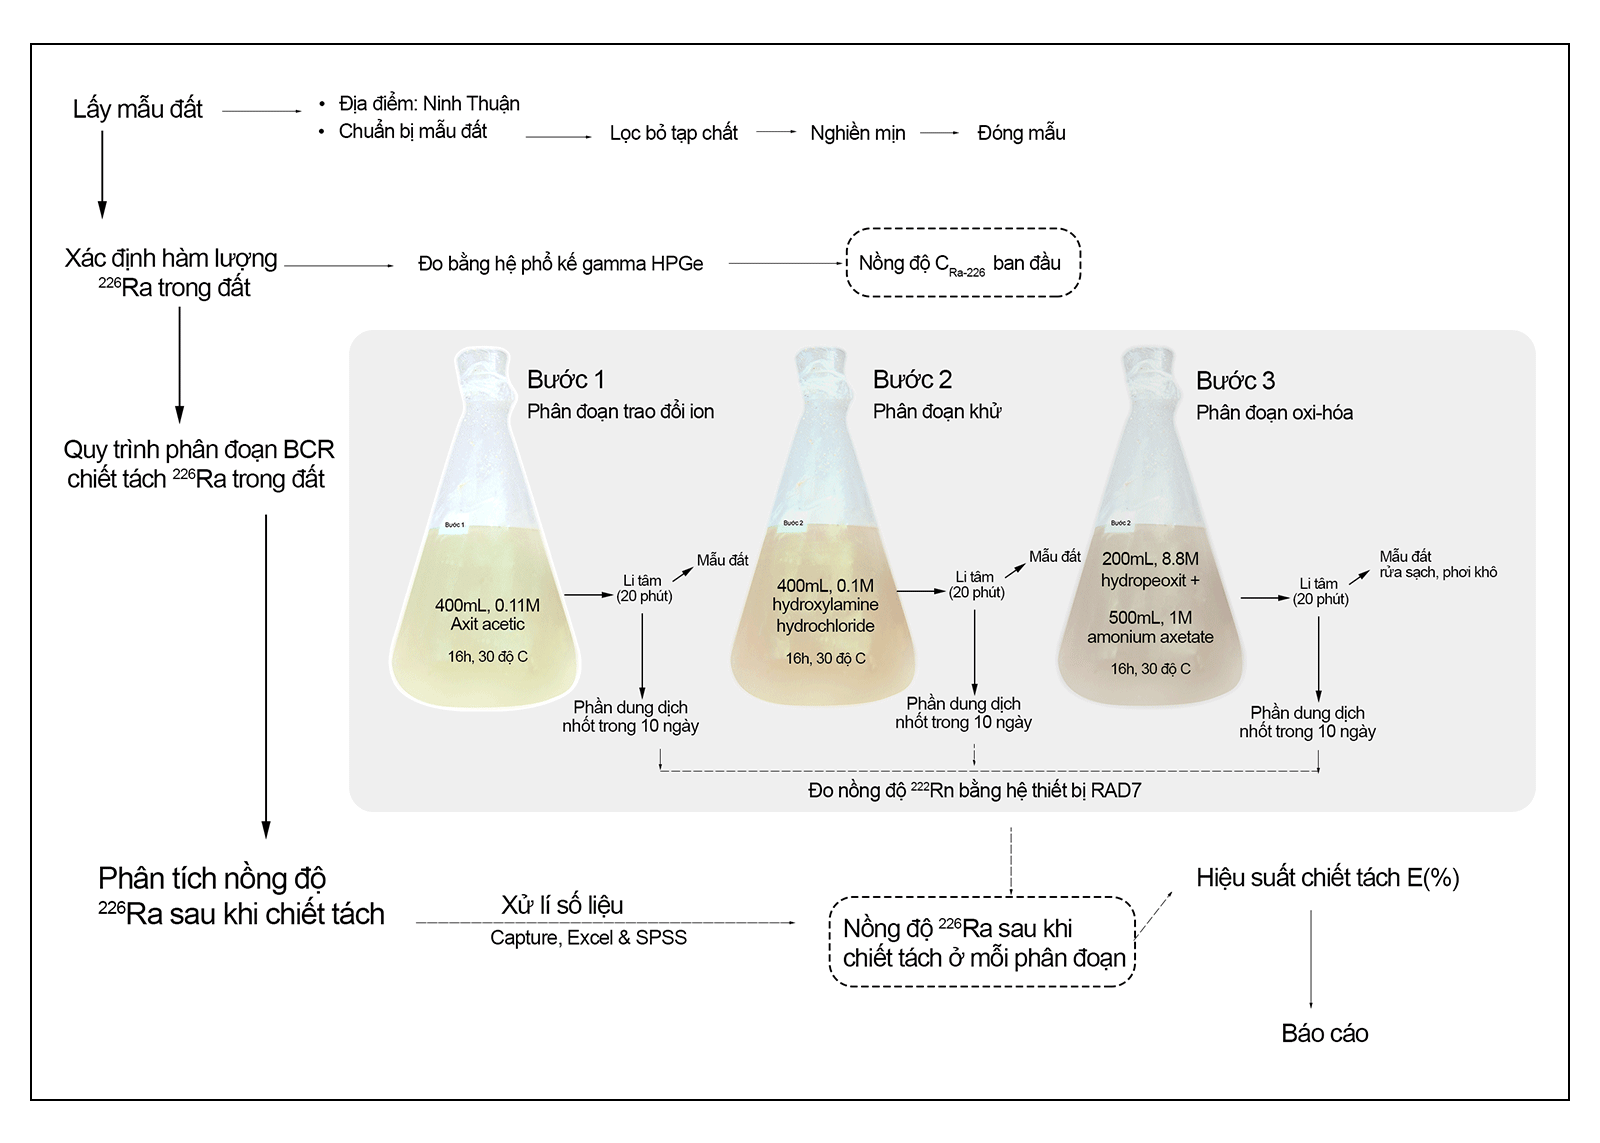
\includegraphics[width=1.1\textwidth]{Image/BCR-Figure1.png}
        \caption{Tóm tắt quy trình xử lí nhiễm bẩn \ce{^226Ra} trong đất}
        \label{figure:DiagramRadiuminSoilBCR}
    \end{figure}


\section{Quy trình lọc tách \ce{^226Ra} trong nước }

\subsection{Xác định nồng độ \ce{^226Ra} trong nước trước khi lọc}
\textbf{Chuẩn bị mẫu}

Các mẫu nước sử dụng cho mục đích nghiên cứu của khóa luận là nước giếng được thu thập tại một số giếng đào thuộc khu vực huyện Ninh Sơn, tỉnh Ninh Thuận. Dùng bộ dụng cụ lấy nước giếng như trong hình ~\ref{figure:EquipmentForMnO2} để lấy mẫu nước giếng. Độ sâu lấy mẫu khoảng 1 m tính từ bề mặt nước. Thể tích mỗi mẫu được lấy là 1 lít.

\begin{figure}[htbp]
    \centering
    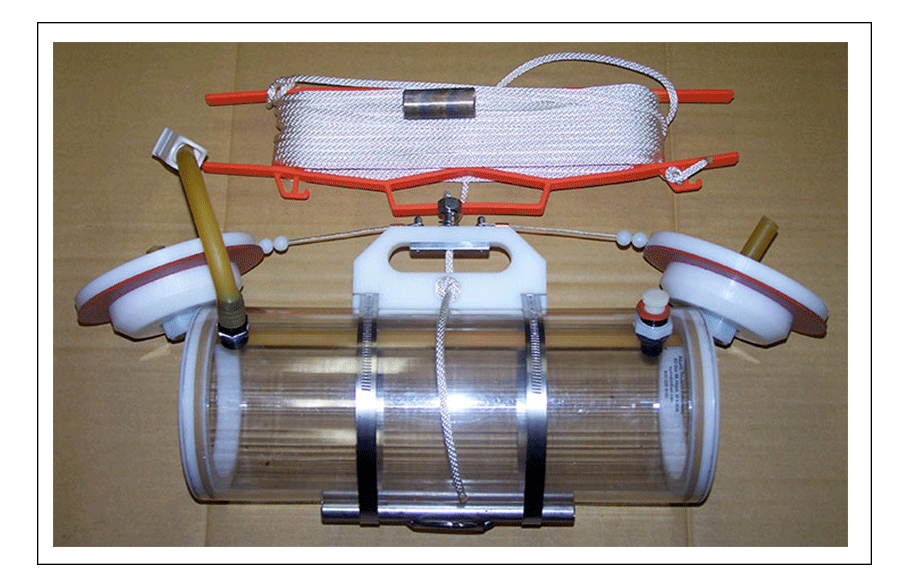
\includegraphics[width=0.8\textwidth]{Image/MnO2-Figure4.png}
    \caption{Dụng cụ lấy mẫu nước}
    \label{figure:EquipmentForMnO2}
\end{figure}

Mẫu sau khi lấy được đo đạc nhanh tại hiện trường một số thông số hóa lý như: nhiệt độ, độ pH. Mỗi mẫu nước sau khi chuyển về phòng thí nghiệm được lấy 250 ml để định lượng \ce{^226Ra}. 

\textbf{Xác định nồng độ \ce{^226Ra} trong nước bằng hệ thiết bị RAD7} 


Mỗi lọ 250 ml nước giếng được khử sạch radon bằng cách bơm đẩy khí ra ngoài lọ. Sau đó, lọ chứa nước giếng được nhốt kín khoảng 10 ngày trước khi xác định nồng độ \ce{^226Ra}. Nồng độ \ce{^226Ra} được xác định thông qua nồng độ radon. Quy trình xác định nồng độ \ce{^226Ra} trong các mẫu nước giếng được trình bày chi tiết trong phần hệ thiết bị RAD7.  

 

 
\subsection{Quy trình điều chế sợi tổng hợp tẩm mangan dioxit}
       
\subsubsection{Thiết bị, dụng cụ và hóa chất}
   
    \textbf{Thiết bị}
        \begin{itemize}
            \item Hệ thiết bị RAD7 của hãng Durridge
            \item Cân điện tử tiểu li: Cân 5 số model PR227/E(2018) của công ty OHAUS, Mỹ (Khối lượng phân tích tối đa 200g, độ chính xác 0,01 mg).
            \item Đèn sấy hồng ngoại của Công ty NTE, Việt Nam (2018), công suất 250W
            \item Bút đo pH điện tử pHTestr30 Waterproof của Công ty OAKTON,  Mỹ, phạm vi đo pH từ –1.00 đến 15.00, ở nhiệt độ từ 0 - 50 (độ C).
            
        \end{itemize}

    \textbf{Dụng cụ và vật liệu}
        \begin{itemize}
            \item Nhiệt kế thủy ngân ($0-100 ^\circ C$, sai số $0.1 ^\circ C$)
            \item Đũa thủy tinh (20cm) và muỗng nhôm.
            \item Cốc thủy tinh chia vạch(50mL, 200mL và 500mL), pipet (2mL), micropipet các  loại của hãng DURAN, Đức.
            \item Lọ thủy tinh (250mL, độ chia nhỏ nhất 50mL) của hãng DURAN, Đức.
            \item Phểu lọc sứ và phểu lọc thủy tinh đường kính phểu 75mm của Genlab, Trung Quốc.
            \item Dây truyền dịch chiều dài 50cm của Công ty Vinamed, Việt Nam.
            \item Bộ giá đỡ thí nghiệm.
            \item Vải sợi tổng hợp thành phần: 90\% polyester, còn lại là sợi polyamid và cotton, kích thước 20cm x 50cm của Công ty Đông Châu, Việt Nam.
            \item Bông gòn 100g của công ty Bông Bạch Tuyết, Việt Nam.
            \item Giấy lọc Whatman loại 1 (11 micron) của hãng Whatman, Mỹ.
        \end{itemize}

    \textbf{Hóa chất}
        \begin{itemize}
            \item \ce{KMnO4} (độ tinh khiết 98.5\%) tinh thể loại P.A, khối lượng 500g của hãng Merck, Mỹ.
            \item Silica gel \ce{SiO2} (độ tinh khiết 95\%), dạng bột mịn (0.5-1.5mm), khối lượng 500g của công ty TRỌNG KHANG , Vietnam.
            \item dung dịch \ce{HCl} (36.5\%-300mL) , hydro peroxit (80\%-300mL)  và dung dịch \ce{NH4OH} (30\%-300mL), dung dịch \ce{NaOH} (3M)  của hãng Merck, Mỹ.
        \end{itemize}
        

    \subsubsection{Các bước thực hiện điều chế sợi tổng hợp tẩm \ce{MnO2}}
        \textbf{Chuẩn bị hóa chất và dụng cụ}
        
        \begin{itemize}
            \item  Lấy 24,06g bột \ce{KMnO4} hòa tan trong nước cất với thể tích 270mL để thu được dung dịch \ce{KMnO4} (0,5M, 300mL).
            \item  Ngâm sợi tổng hợp với dung dịch \ce{HCl} (20mL - 5\%), hydro peroxit (10mL-80\%) trong 200mL nước cất, ở nhiệt độ phòng trong thời gian 2h. Thực hiện bước này nhằm loại bỏ hóa chất nhuộm vải, và các nấm móc có trong vải sợi, và nhằm hạn chế thấp nhất các điều kiện bên ngoài tác động đến các liên kết của sợi vải.\\
        \end{itemize}



        \textbf{Bước 1}: Ngâm sợi tổng hợp  polyester trong dung dịch 0,5M \ce{KMnO4} trong 2h ở nhiệt độ khoảng $50 - 65 ^\circ C$, 20g chất nền \ce{SiO2} . \ce{KMnO4} bị oxy hóa tạo thành \ce{MnO2} gắn lên bề mặt sợi acrylic và chất nền \ce{SiO2}. Vấn đề cần lưu ý là trong quá trình phản ứng, cần điều chỉnh và ổn định nhiệt độ dung dịch không vượt quá $ 65 ^\circ C$. Sau 1h, sợi acrylic chuyển dần sang màu cam và cuối cùng chuyển thành màu đen (\ce{MnO2}) (trong hình ~\ref{figure:MauVaiBeforeAfterMnO2}), do \ce{KMnO4} bị oxi hoá phân huỷ nhiệt  tạo thành \ce{MnO2} theo phương trình phản ứng:

        \begin{equation*}
            \ce{2KMnO4 ->[$t^o$] K2MnO4 + MnO2 + O2 ^}
        \end{equation*}

        \begin{figure}[htbp]
            \centering
            \includegraphics[width=0.95\textwidth]{Image/MnO2-Figure6.png}
            \caption{Mẫu vải sợi tổng hợp polyester trước và sau khi tẩm \ce{MnO2}}
            \label{figure:MauVaiBeforeAfterMnO2}
        \end{figure}

         
        \textbf{Bước 2}: Sợi sau khi tẩy được lấy ra, rửa sạch bằng nước cất, lắc nhẹ để loại bỏ \ce{KMnO4} dư và phần \ce{MnO2} chưa được hình thành liên kết với sợi
        
        \textbf{Bước 3:} Thực hiện sấy khô sợi ở $ 80^\circ C$, trong vòng 30 phút.



\subsubsection{Các bước lọc \ce{^226Ra} trong nước bằng sợi tổng hợp tẩm \ce{MnO2}}        
        \textbf{Bước 1} Chuẩn bị

        \begin{itemize}
            \item Phểu lọc được bọc lót cẩn thận với 3 tấm lọc: Lớp lọc trên cùng là vải sợi tẩm \ce{MnO2} độ dày 5mm, phần giữa là bông gòn và giấy lọc, dưới cùng là vải sợi tẩm \ce{MnO2} độ dày 10mm. 
            \item Các dụng cụ lọc được sắp đặt như trong hình ~\ref{figure:QuyTrinhlocMnO2}
            \item Các mẫu nước được lọc thô bằng vải mỏng để loại bỏ cặn. Sau đó, điều chỉnh pH của mẫu nước ở khoảng từ 7-7.5 bằng dung dịch \ce{HCl} (5\%) và \ce{NH4OH} (10\%), theo ~\cite{MnO2:WillardS.Moore} trong khoảng pH trên thì hiệu suất hấp thụ \ce{^226Ra} của \ce{MnO2} là cao và tối ưu. Sau đó, mẫu nước được đựng trong bình lọc ở thể tích 250mL
        \end{itemize}  

        \textbf{Bước 2} Lọc nước
            \begin{itemize}
                \item Thực hiện lọc mẫu nước trong vòng từ 30-45 phút, ở nhiệt độ phòng từ 28-30 (độ C). Lưu ý, phải điều chỉnh tốc độ dòng chảy của nước ổn định ở  2 (mL/phút) và nhiệt độ ổn định, hạn chế tác động ngoại lực từ bên ngoài lên phểu lọc để nước thấm đều tấm lọc, và hạn chế nước tràn ra ngoài. Hình ~\ref{figure:MnO2SoDoLoc}, thể hiện sơ đồ bố trí thiết bị - dụng cụ lọc mẫu nước bằng sợi tổng hợp tẩm \ce{MnO2}. 
                \item Nước sau khi lọc được đựng trong lọ thủy tinh 250mL và nhốt trong vòng 10 ngày, sau đó thực hiện đo trên hệ thiết bị RAD7.
            \end{itemize}


        \textbf{Bước 3} Đo mẫu phân tích:
         Mẫu nước sau khi được nhốt trong vòng 10 ngày, thực hiện đo trên hệ thiết bị RAD7 trong vòng 4-5h. Dữ liệu đo thể hiện trong phần mềm CAPTURE version 5.7 của hãng Durridge.  Mẫu nước sau khi đo được rửa giải bằng dung dịch hydro peroxit và dung dịch \ce{HCl} (35.6\%), cuối cùng được trung hòa bằng dung dịch \ce{NaOH}. 
            
       
        \begin{figure}
            \centering
            \caption{Sơ đồ bố trí thiết bị và dụng cụ lọc mẫu nước }
            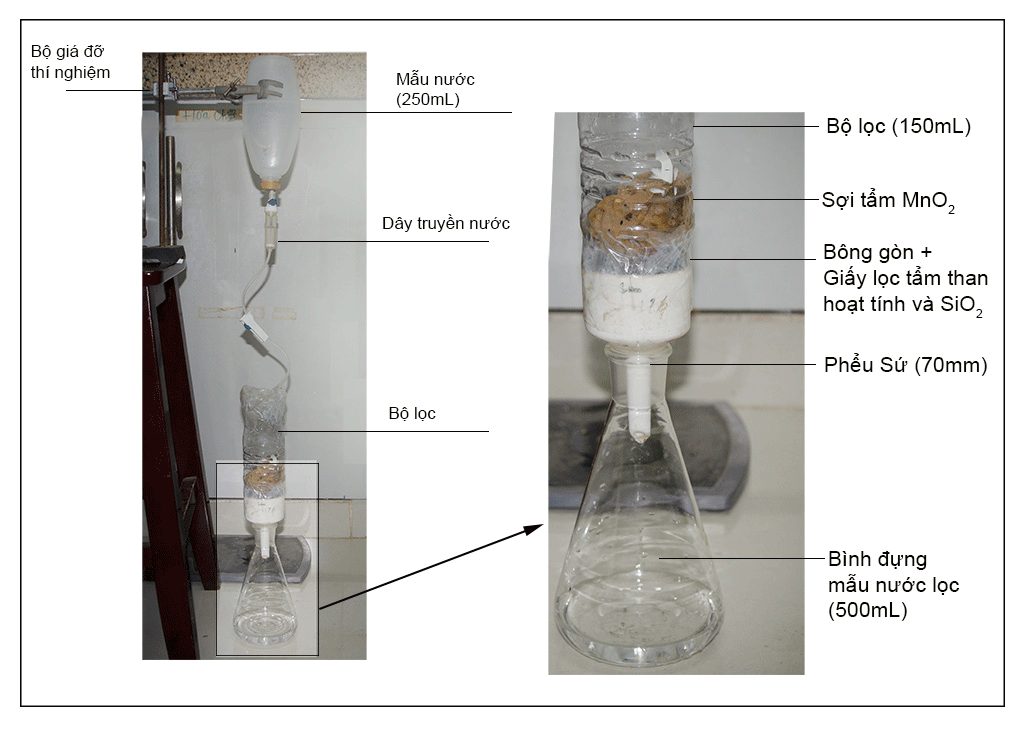
\includegraphics[width=0.85\textwidth]{Image/MnO2-Figure5.png}
            \label{figure:MnO2SoDoLoc}
        \end{figure}


    \subsubsection{Phân tích nồng độ \ce{^226Ra} sau khi lọc tách bằng sợi tổng hợp tẩm \ce{MnO2}}

         \textbf{Hiệu suất quy trình lọc \ce{^226Ra}} :
         
         Hiệu suất quy trình lọc tách \ce{226Ra} trong mẫu nước bằng  sợi tổng hợp \ce{MnO2} được tính theo công thức: 
            \begin{equation}
                E (\%) = \qty(1 - \dfrac{C_2}{C_1}).100\%
            \end{equation}

           Sai số phần trăm hấp thụ 
           \begin{equation}
            \sigma_E = \qty(\dfrac{C_2}{C_1}).\sqrt{\qty(\dfrac{\sigma_{C_1}}{C_1})^2+\qty(\dfrac{\sigma_{C_2}}{C_2})^2}
        \end{equation}

        Trong đó: 
        \begin{itemize}
            \item $C_1 \pm \sigma_{C_1}(Bq/m^3)$: Nồng độ \ce{^226Ra} trong mẫu nước trước khi lọc hấp thụ.  
            \item $C_2  \pm \sigma_{C_2} (Bq/m^3)$: Nồng độ \ce{^226Ra} trong mẫu nước sau khi lọc hấp thụ bằng sợi \ce{MnO2}.
        \end{itemize}
 


    \textbf{ Liều hiệu dụng hằng năm do uống nước chứa \ce{^222Rn}  và \ce{^226Ra}}

      Liều hiệu dụng hằng năm $D_w$ (Sv) mà một người nhận được từ uống nước chứa đồng vị \ce{^222Rn} và \ce{^226Ra} và sai số được tính toán theo công thức:  
      \begin{align}
          &D_w = \varepsilon. V. C_w\\
          &\sigma_{D_w} = \varepsilon.V.\sigma_{C_w} \varepsilon = \dfrac{E}{C}.\sigma_{C_w}
      \end{align}
      Trong đó: 
      \begin{itemize}
          \item $\varepsilon$ là hệ số chuyển đổi liều hiệu dụng trên một đơn vị nồng độ phóng xạ, với \ce{^222Rn}: giá trị $\varepsilon= 10^{-8}$ (Sv/Bq), trong trường hợp \ce{^226Ra} thì giá trị $\varepsilon  = 2,8 \times 10^{-7} $ (Sv/Bq)
          \item $C_w \pm \sigma_{C_w}  (Bq/m^3)  $ là nồng độ tuyệt đối của  \ce{^222Rn}  hoặc \ce{^226Ra}
          \item V là thể tích mỗi người uống trung bình một năm. Từ các số liệu thống kê, trong một ngày một người uống  uống 2 lít nước thì giá trị $V  = 2.10^{-3} \times 365 = 0,73 (m^3) $ 
      \end{itemize}
     Theo báo cáo của UNSCEAR (2000), liều hiệu dụng trung bình toàn cầu do uống nước chứa \ce{^222Rn} khoảng 2 ($\mu Sv$/năm), và nước  chứa \ce{^226Ra} khoảng 8  ($\mu Sv$/năm).  Cơ quan bảo vệ môi trường Hoa Kì, USEPA, đã đưa ra mức giới hạn nồng độ  \ce{^222Rn} và \ce{^226Ra} trong nước lần lượt là 11,1 (Bq/L) và 0,185 (Bq/L) ~\cite{Thesis:HNPThu}. 
     
     
      
     Hình ~\ref{figure:DiagramRadiuminSoilBCR}, mô tả tóm tắt quy trình xử lí nhiễm bẩn \ce{^226Ra} trong nước bằng quy trình hấp thụ \ce{^226Ra} trên sợi tổng hợp tẩm \ce{MnO2}

     \begin{figure}[htbp]
         \centering
         \includegraphics[width=0.85\textwidth]{Image/MnO2-Figure3.png}
         \caption{Tóm tắt quy trình xử lí nhiễm bẩn \ce{^226Ra} trong nước}
         \label{figure:MnO2SoDoTomTat}
     \end{figure}
 
       
 

        
        
        
        

      Liều hiệu dụng hằng năm $D_w$ (Sv) mà một người nhận được từ uống nước chứa đồng vị \ce{^222Rn} và \ce{^226Ra} và sai số được tính toán theo công thức:  

      \begin{align}
          &D_w = \varepsilon. V. C_w\\
          &\sigma_{D_w} = \varepsilon.V.\sigma_{C_w} \varepsilon = \dfrac{E}{C}.\sigma_{C_w}
      \end{align}
      Trong đó: 

      Các hoạt động khai thác quặng, dầu và khí tự nhiên, các mạch nước ngầm gây ra phơi nhiễm phóng xạ tự nhiên trong môi trường. Điều này dẫn đến hàm lượng phóng xạ tại các địa điểm diễn ra các hoạt động trên có khả năng vượt ngưỡng an toàn phóng xạ cho phép. Trong số các đồng vị phóng xạ, 226Ra được xem là một đồng vị quan trọng do có chu kỳ bán rã dài, khả năng ion hóa cao và có tính chất hóa học tương đồng với nhiều kim loại kiềm thổ khác trong đất. Các đồng vị con cháu của 226Ra cũng có có khả năng ion hóa cao, đặc biệt 226Ra còn sinh ra 222Rn, một đồng vị phóng xạ dạng khí có khả năng phân tán vào môi trường rất cao. Trên thế giới, có nhiều công trình nghiên cứu cho thấy, chất thải tự nhiên do các hoạt động khai thác quặng, dầu khí,…gây ra có hàm lượng phóng xạ rất cao trong đất, có vùng lên đến 1000 kBq/kg [Al-Masri, 2003; Agbalagba, 2013; Al Attar, 2015; Bajoga, 2015].
      
      \begin{itemize}
          \item $\varepsilon$ là hệ số chuyển đổi liều hiệu dụng trên một đơn vị nồng độ phóng xạ, với \ce{^222Rn}: giá trị $\varepsilon= 10^{-8}$ (Sv/Bq), trong trường hợp \ce{^226Ra} thì giá trị $\varepsilon  = 2,8 \times 10^{-7} $ (Sv/Bq)
          \item $C_w \pm \sigma_{C_w}  (Bq/m^3)  $ là nồng độ tuyệt đối của  \ce{^222Rn}  hoặc \ce{^226Ra}
          \item V là thể tích mỗi người uống trung bình một năm. Từ các số liệu thống kê, trong một ngày một người uống  uống 2 lít nước thì giá trị $V  = 2.10^{-3} \times 365 = 0,73 (m^3) $ 
      \end{itemize}

     Theo báo cáo của UNSCEAR (2000), liều hiệu dụng trung bình toàn cầu do uống nước chứa \ce{^222Rn} khoảng 2 ($\mu Sv$/năm), và nước  chứa \ce{^226Ra} khoảng 8  ($\mu Sv$/năm).  Cơ quan bảo vệ môi trường Hoa Kì, USEPA, đã đưa ra mức giới hạn nồng độ  \ce{^222Rn} và \ce{^226Ra} trong nước lần lượt là 11,1 (Bq/L) và 0,185 (Bq/L) ~\cite{Thesis:HNPThu}. 
     
     
% \setcounter{chapter}{2}
% Setting Chapter 3

\chapter{Thực nghiệm và kết quả thảo luận}
    \section{Kết quả phân tích \ce{^226Ra} trong đất}
    \section{Kết quả phân tích \ce{^226Ra} trong nước}
        \subsection{Đánh giá về khả năng hấp thụ mangan dioxit trên sợi vải tổng hợp}
        \subsection{Tính toán liều hiệu dụng hằng năm do uống nước chứa \ce{^222Rn}  và \ce{^226Ra}}
            Liều hiệu dụng hằng năm $D_w$ (Sv) mà một người nhận được từ uống nước chứa đồng vị \ce{^222Rn} và \ce{^226Ra} và sai số được tính toán theo công thức:  
            
            \begin{align}
                &D_w = \varepsilon. V. C_w\\
                &\sigma_{D_w} = \varepsilon.V.\sigma_{C_w} \varepsilon = \dfrac{E}{C}.\sigma_{C_w}
            \end{align}

            Trong đó: 
            \begin{itemize}
                \item $\varepsilon$ là hệ số chuyển đổi liều hiệu dụng trên một đơn vị nồng độ phóng xạ, với \ce{^222Rn}: giá trị $\varepsilon= 10^{-8}$ (Sv/Bq), trong trường hợp \ce{^226Ra} thì giá trị $\varepsilon  = 2,8 \times 10^{-7} $ (Sv/Bq)
                \item $C_w \pm \sigma_{C_w}  (Bq/m^3)  $ là nồng độ tuyệt đối của  \ce{^222Rn}  hoặc \ce{^226Ra}
                \item V là thể tích mỗi người uống trung bình một năm. Từ các số liệu thống kê, trong một ngày một người uống  uống 2 lít nước thì giá trị $V  = 2.10^{-3} \times 365 = 0,73 (m^3) $ 
            \end{itemize}
           Theo báo cáo của UNSCEAR (2000), liều hiệu dụng trung bình toàn cầu do uống nước chứa \ce{^222Rn} khoảng 2 ($\mu Sv$/năm), và nước  chứa \ce{^226Ra} khoảng 8  ($\mu Sv$/năm).  Cơ quan bảo vệ môi trường Hoa Kì, USEPA, đã đưa ra mức giới hạn nồng độ  \ce{^222Rn} và \ce{^226Ra} trong nước lần lượt là 11,1 (Bq/L) và 0,185 (Bq/L) ~\cite{Thesis:HNPThu}. 
           

    
\clearpage
% \chapter*{Kết luận và kiến nghị}
\clearpage
% --------- Tai Lieu Tham Khao 
\addcontentsline{toc}{chapter}{Tài liệu tham khảo}
\chapter*{Tài liệu tham khảo}

\printbibliography[keyword=Vietnamese,heading=subbibintoc,title=Tiếng Việt]
\printbibliography[keyword=English,heading=subbibintoc,title=Tiếng Anh]
\printbibliography[keyword=Online,heading=subbibintoc,title=Trang Website]
\end{document}


